% Use only LaTeX2e, calling the article.cls class and 12-point type.

\documentclass[12pt]{article}

% Users of the {thebibliography} environment or BibTeX should use the
% scicite.sty package, downloadable from *Science* at
% http://www.sciencemag.org/authors/preparing-manuscripts-using-latex 
% This package should properly format in-text
% reference calls and reference-list numbers.

\usepackage{scicite}

\usepackage{times}

\usepackage{lscape} 

%setup for commenting during editing
\usepackage{xcolor}
\newcommand{\tom}[2]{{\color{red}{#1}}\footnote{\textit{\color{red}{#2}}}}
\newcommand{\josh}[2]{{\color{blue}{#1}}\footnote{\textit{\color{blue}{#2}}}}

% for adjusting the sizes of tables
\usepackage{adjustbox}
% for setting up equations
\usepackage{amsmath}

% The preamble here sets up a lot of new/revised commands and
% environments.  It's annoying, but please do *not* try to strip these
% out into a separate .sty file (which could lead to the loss of some
% information when we convert the file to other formats).  Instead, keep
% them in the preamble of your main LaTeX source file.


% The following parameters seem to provide a reasonable page setup.

\topmargin 0.0cm
\oddsidemargin 0.2cm
\textwidth 16cm 
\textheight 21cm
\footskip 1.0cm


%The next command sets up an environment for the abstract to your paper.

\newenvironment{sciabstract}{%
\begin{quote} \bf}
{\end{quote}}



% Include your paper's title here

\title{Context-dependent host-microbe interactions in stochastic environments} 


% Place the author information here.  Please hand-code the contact
% information and notecalls; do *not* use \footnote commands.  Let the
% author contact information appear immediately below the author names
% as shown.  We would also prefer that you don't change the type-size
% settings shown here.

\author
{Joshua C. Fowler,$^{1\ast}$ Shaun Ziegler,$^{2}$ Kenneth D. Whitney,$^{2}$\\
	 Jennifer A. Rudgers,$^{2}$ Tom E. X. Miller $^{1}$\\
\\
\normalsize{$^{1}$Rice University, Department of BioSciences, Houston, TX, 77005}\\
\normalsize{$^{2}$University of New Mexico, Department of Biology, Albuquerque, NM, 87131}\\
\\
\normalsize{$^\ast$To whom correspondence should be addressed; E-mail:  jcf3@rice.edu.}
}

% Include the date command, but leave its argument blank.

\date{}



%%%%%%%%%%%%%%%%% END OF PREAMBLE %%%%%%%%%%%%%%%%



\begin{document} 

% Double-space the manuscript.

\baselineskip24pt

% Make the title.

\maketitle 



% Place your abstract within the special {sciabstract} environment.

\begin{sciabstract}
	ABSTRACT: Microbial symbioses are ubiquitous in nature, yet 


\end{sciabstract}



% In setting up this template for *Science* papers, we've used both
% the \section* command and the \paragraph* command for topical
% divisions.  Which you use will of course depend on the type of paper
% you're writing.  Review Articles tend to have displayed headings, for
% which \section* is more appropriate; Research Articles, when they have
% formal topical divisions at all, tend to signal them with bold text
% that runs into the paragraph, for which \paragraph* is the right
% choice.  Either way, use the asterisk (*) modifier, as shown, to
% suppress numbering.

\section*{Main Text}

Along with increases in average temperatures, global climate change is characterized by increases in the variability of precipitation events and the frequencies of extreme weather events \cite{IPCC2012managing,seneviratne2012changes,stocker2013technical}.
Discerning the effects of increasing environmental variability on population dynamics is therefore a key objective of global change ecology. 
\tom{Population responses to variability are likely shaped by species' life history \cite{pfister1998patterns,morris2008longevity,saether2013life} with important consequences for conservation and management \cite{menges2000applications}, but the impact that biotic interactions have on these responses is unclear.}{This sentence feels out of place here - I would go straight to ``classic theory''.}

Classic theory predicts that long-term population growth rates (equivalently, population mean fitness) will decline under increased environmental variability due to negative effects of bad years that outweigh the positive effects of good years (a consequence of nonlinear averaging) \cite{lewontin_population_1969,tuljapurkar_population_1982}.
For example, in unstructured populations, the long-term stochastic growth rate in fluctuating environments ($\lambda_s$) will always be less than the growth rate averaged across environments ($\overline{\lambda}$) by an amount proportional to the environmental variance ($\sigma^2$): 
\begin{equation}
	 log(\lambda_s)  \approx log(\overline{\lambda}) - \frac{\sigma^2}{2\overline{\lambda}^2}
\end{equation}

Populations structured by size or stage are expected to similarly experience negative effects of variability \cite{cohen1979comparative,tuljapurkar2013population}.
Thus, there are two pathways to increase population viability in a stochastic environment: increasing the mean growth rate and/or dampening temporal fluctuation in growth rates, also called variance ``buffering''.

Given the potential for negative fitness consequences of increasing environmental stochasticity under global change, a large body of research has examined the properties of species or their environments that can amplify or dampen demographic fluctuations, including life history traits such as longevity \cite{morris2008longevity}, correlations between vital rates \cite{compagnoni2016effect}, transient shifts in stage structure \cite{ellis2013role}, and the degree of environmental autocorrelation \cite{tuljapurkar1980population,fieberg2001stochastic}. 
Much less is known about how biotic interactions modulate responses to demographic variability \cite{hilde_demographic_2020}. 
%Because practically all species host symbiotic microorganisms that impact growth and performance \cite{rodriguez2009fungal,mcfall2013animals}, we investigated the potential for microbial symbionts to provide variance buffering for their hosts and how these responses may change under future climate change.

Practically all multi-cellular species host symbiotic microorganisms that impact growth and performance \cite{rodriguez2009fungal,mcfall2013animals}, and many of these are transmitted via reproduction from maternal hosts to offspring \cite{funkhouser2013mom}.
The process of vertical transmission links the fitness of hosts and symbionts together, leading to the expectation of host-symbiont mutualism, else the symbionts cause their host to be selected out of the population \cite{ewald1987transmission,fine1975vectors}. 
\tom{Many}{The rest of this paragraph seems to lose the thread of vertical transmission.} mutualistic microbes provide their hosts with protection from environmental stresses including drought, extreme temperatures, and enemies \cite{russell2006costs,brownlie2009symbiont,kivlin2013fungal,corbin2017heritable,hoadley2019host}. 
Such defensive mutualisms are intrinsically context-dependent, because the magnitude of benefits to host organisms depends on the type and degree of threat \cite{chamberlain2014context}. 
In a stochastic environment, the strength of host-symbiont mutualism can vary through time as the environment fluctuates \cite{jordano1994spatial,billick2003relative}. 
Therefore, \tom{context-dependent symbioses}{I don't think the symbiosis is context-dependent -- the endophytes are always in there. It's the mutualism that is context dependent.} may buffer variability by providing benefits to their hosts during years with harsh conditions, while being neutral or even costly during years with benign conditions, reducing the frequency of extreme years experienced by symbiotic hosts relative to non-symbiotic hosts. 
Variance buffering is a \tom{previously unexplored}{Not just previously unexplored but basically inaccessible because there are no long-term experiments on microbial symbioses -- would be good to make this point somehow.} mechanism by which context-dependent symbionts may act as mutualists to their hosts, in addition to elevating average fitness, which may come to be of increasing importance in a more variable future \cite{rudgers2020climate}. 

Using data from a unique, long-term symbiont-removal experiment, we tested the hypothesis that context-dependent benefits of symbiosis buffer hosts from the fitness consequences of environmental variability by (i) quantifying the effects of symbiosis on the mean and variance of host vital rates (survival, growth and reproduction), (ii) quantifying the relative contribution of mean and variance effects on long-term population fitness, (iii) and used simulations to explore the consequences of variance buffering under increased variability.\tom{}{I think the life history trait comparisons is an important addition to this list.}
Initiated in 2007 in south-central Indiana, USA with seven grass species that host \emph{Epichlo\"{e}} fungal endophytes, the experiment consisted of annually censused plots planted with either naturally symbiotic plants (E+) or those which have had their symbionts experimentally removed  via a heat treatment (E-) (See SM for a full list of species and experimental methods).\tom{}{If you are going to use symbiotic/non-symbiotic then maybe S+ and S-. ``E'' makes more sense if you are talking specifically about endophytes.}
\emph{Epichlo\"{e}} fungi are specialized symbionts growing intercellularly in the aboveground tissue of at least 30\% of cool-season (C3) grass species \cite{leuchtmann1992systematics}.
They are primarily transmitted vertically from maternal plants through seeds \cite{cheplick2009ecology,rudgers2009fungus}.
The fungi produce a variety of alkaloids, which have been demonstrated to provide hosts with protection against herbivory \cite{brem2001epichloe} drought stress \cite{cheplick2004recovery,kannadan2008endophyte,decunta2021systematic}.\tom{}{I don't think alkaloids have ever been mechanistically connected to drought, so you could re-word this to say that endophytes confer protection against herbivory and drought, likely through synthesis of alkaloids.}

The data from this long-term experiment are uniquely suitable for detecting fitness benefits of microbial symbiosis that arise through variance buffering. 
During each annual census, we collected demographic data on the vital rates (survival, growth, and reproduction) of all individuals, and we added new recruits to the census. 
Each of the 14 census years is a sample of interannual climatic variation.
We fit vital rate models as hierarchical Bayesian generalized linear mixed models using Rstan \cite{rstan2022}, allowing us to isolate endophyte effects on vital rate means and variances, borrow strength across species for some variance components, and propagate uncertainty from the vital rate estimates to our population model \cite{elderd2016quantifying}. 
We then parameterized stochastic matrix population models for each of the seven grass host species from the vital rate regressions to comprehensively quantify endophyte effects on fitness and decompose the overall effect of the symbiosis into contributions through mean vital rates, variance in vital rates, and their interaction (see Supplemental Material for a full description of statistical methods).

Across seven host species, eight vital rates, 14 years, and 16,789 individual host plants, we found that endophyte symbiosis consistently altered the mean and variance of host vital rates. 
Endophytes had a positive effect on the mean for $36$ out of $56$ host species--vital rate combinations, and effects were particularly strong for host survival, growth and germination \tom{(Fig. 1A)}{Nice figure- but I wonder if we could find more attractive line drawings for the grasses.}.
Endophytes also consistently reduced inter-annual variance for the majority of host species and vital rates ($37$ out of $56$ host species--vital rate combinations; Fig. 1A), consistent with the hypothesis of variance buffering.\tom{}{Need to say more, here and in the caption, about the quantities are shown in Fig 1. ``mean standardized effect size'' is ambiguous.} 
The relative magnitude of symbiont effects on means and variances was idiosyncratic across species and across vital rates.
For example, endophytes modestly increased mean adult survival (Fig. 1C )and reduced variance (Fig. 1D) for \emph{Festuca subverticillata}, while for \emph{Poa alsodes}, variance buffering was more apparent in seedling growth and in inflorescence production (Fig 1E). 
Interestingly, there were also certain vital rates that showed costs of endophyte symbiosis. 
Symbiotic individuals of \emph{A. perennans} grew at a higher rate between censuses than those without endophytes (Fig. 1B), yet endophytes also reduced mean germination rates. 
Similarly, endophyte partnership led to greater variance in seedling growth for \emph{Elymus villosus} and \emph{Festuca subvertcillata}.
 
Not all vital rates contribute equally to fitness, so we used stochastic matrix models (where tiller number was the integer-valued state variable) to integrate the diverse effects described above into comprehensive measures for the mean and variance of host fitness.
We found that, on average across host species, endophyte-symbiotic populations experienced a 9.2 \% increase in mean fitness $\overline{\lambda}$. 
Our hierarchical Bayesian analysis, which propagates uncertainty from the underlying data through model predictions, indicates 92.8\% confidence that endophytes increased $\overline{\lambda}$ (Fig. 2A).\tom{}{For Fig 2, can axis labels be changed to ``Symbiosis effect on''?}
The coefficient of variation of $\lambda$, reflecting inter-annual variability in fitness, was 38.9\% lower in endophyte-symbiotic populations than endophyte-free populations, (with 86.2\% confidence that the endophyte effect was negative) (Fig. 2B).
For some host species, the coefficient of variation was  reduced by as much as 168.2\% (\emph{P. alsodes}) and 172.6\% (\emph{F. subverticillata}), while for others, effects were much smaller (5.5\% and 16.3\% reductions for\emph{E. villosus} and \emph{A. perennans} respectively), or even slightly positive  (27.1\% increase for \emph{E. virginicus}).
When the two mechanisms are considered together, none the host-symbiont pairings are antagonistic (i.e. with endophytes that both decrease mean and increase variance) (Fig. 2C) \tom{suggesting that differences between hosts' mean and variance effects may reflect strategies which maximize their fitness}{Do not follow.}. 

Having documented positive fitness effects of endophyte symbiosis via mean benefits and / or variance buffering, we next asked about the relative importance of those two pathways of host-symbiont mutualism for the stochastic growth rate $\lambda_{S}$.
We decomposed the overall effect of the symbiosis on $\lambda_{S}$ into contributions from mean and variance buffering effects.
To do this, we estimated $\lambda_{S}$ incorporating both mean and variance buffering effects, as well as for mean effects alone, for variance effects alone, and for models without any effects of endophytes. 
We ran each simulation for 1000 years by randomly sampling from the annual transition matrices observed over the course of the experiment, discarding the first 100 years to remove transient dynamics, and calculated the mean of growth rates.  
Sampling observed transition matrices leads to models which realistically capture interannual variation by preserving correlations between individual vital rates.\tom{}{cite Metcalf et al. 2015 Statistical modelling of annual variation for inference on stochastic population dynamics using Integral Projection Models}
Overall, we found strong that, on average across host species, fungal endophytes are mutualists (100\% certainty of a positive total effect on $\lambda_{S}$ \tom{across species}{We need to communicate what exactly this is a little better.}) (Fig. 3).
Under observed conditions, contributions to $\lambda_{S}$ come from both mean and variance buffering effects, with effects on the mean that are 4.17 times greater on average than contributions from variance buffering. 
Yet, for two species (\emph{A. perennans} and \emph{P. syvestris}) contributions from variance buffering are greater than mean effects (Fig. S6). 
\tom{Noteably, the three host species for which the mutualism was weakest (\emph{Elymus villosus}, \emph{Elymus virginicus}, and \emph{Poa sylvestris}) (Fig. 2C) were the only hosts for which we have observed evidence of horizontal transmission (Table S2), in line with theoretical expectations for the role of transmission in the evolution of symbiotic mutualisms \cite{fine1975vectors,afkhami2008symbiosis}.}{Save for traits section?}

\tom{Life history variation is a potential explanation differences in strategy across species. }{This paragraph is great - needs to be set up better in intro.}
Long-lived host species, those on the slow end of the slow-fast life history continuum, are expected to be less sensitive to environmental variability \cite{murphy1968pattern}, a pattern which has empirical support across plants \cite{compagnoni2021herbaceous} and animals \cite{le2022life}. 
We would expect species that have a \tom{slower life history}{I think you need to define this better. What makes a life history ``slow''?} to benefit less from the variance buffering effects of endophytes. 
To test this, we collected trait data for each host species, calculating demographic life history traits from \tom{matrix models}{E+ or E-?} using the Rage package (generation time, longevity, mean life expectancy, and net reproductive)\cite{jones2022rcompadre} and collating other traits from the literature (seed size) and from the experimental plots (maximum observed age). 
These traits reflect a trade-off between producing fewer, larger offspring that are better able to persist through environmental variability and producing many smaller offspring with a lower per-capita chance of success \cite{rees1996evolutionary,moles2004seedling}. 
In general, host species with trait values representing faster life history strategies experience a stronger buffering effect from endophytes (Fig 4). 
For example, variance buffering was stronger for host species with smaller seeds (Fig, 4G) and shorter generation times (Fig. 4F).
This supports the hypothesis that species with faster life-histories benefit more from symbiont-mediated variance buffering, \tom{however drawing firm conclusions about the role that variance-buffering symbioses can play as a part of species' life history strategies generally is difficult given the relatively limited number of hosts. }{I understand the need for caution, but there has got to be a less deflating way to say this.}
These hosts and their vertically-transmitted symbionts share close evolutionary history with traits spanning a relatively narrow range of values.
Our understanding of the role of symbiosis in life history theory would be improved by testing for variance buffering effects across taxonomic groups \cite{jeschke2009roles}.
\josh{However, the lack of relationship may be explained partly by the inclusion of \emph{L. arundinaceum}, which has exceptionally long longevity compared to the other host species. 
\emph{L. arundinaceum} is a common model species for studying the effects of \emph{Epichlo\"{e}} fungal endophyte symbiosis, but is a non-native invasive species in much of North America \cite{schardl2005epichloe}. }{This could maybe be dropped? I wrote this earlier, but after looking at the data longer, I ended up not doing to the regressions separately, and this sentence kind of contradicts the preceding sentences. But I think there is still some value in describing how weird LOAR is in terms of being hugely mean effect driven, and being non-native.}\tom{}{This is something that would be a natural component of a discussion section in, say, Ecology. Not sure it is a strategic addition for Science.}

\tom{We next used simulations to assess how contributions from mean effects and variance buffering change under increased variability, a key prediction of climate change.}{This will flow better if it follows the description of ``all years'' results. We might also think about just showing 2 and 6 extreme years, which would simplify this figure.}
Under the regime of environmental variability observed during the course of the experiment, endophyte effects on mean population growth rates are the primary contribution to mutualistic outcomes.
To simulate increased variability, we repeated the estimation of $\lambda_{S}$ under three scenarios of increasing variability, choosing the transition matrices of the most extreme six, four, and two years. 
These treatments increased the \tom{standard deviation}{of what?} by $1.3$, $1.6$, and $2.1$ times compared to the ambient scenario, while maintaining equivalent mean growth rates (less than $2.3\%$ difference between simulation treatments)(See SM; Fig. S7).
Under increased variability, endophyte symbiosis provides stronger mutualistic benefits (Fig. 3), driven by increasing contributions from the variance buffering mechanism (from 24.4\% to 66.2\% contribution from variance buffering between the ambient and most extreme scenarios), while the overall effect of the symbiosis increased by more than 130 \% under increased variance.
This result suggests that mutualism with \emph{Epichlo\"{e}} endophytes in general, and their variance buffering effect in particular, will take on increased importance for their hosts in a more variable climate future.

\tom{}{We can talk more about it, but I might reduce this paragraph and incorporate its key points into the sections above. For example, where you first describe the buffering result, you can say that climate-explicit analyses indicate that S+ populations are less sensitive to drought conditions than S- for five of seven species, then reference the supplement.}To explore the climate sensitivities responsible for endophytes' ability to buffer against stochasticity, we constructed climate-explicit population models with annual and growing season drought indices (12 and 3 month SPEI respectively) (See Supplemental Methods). 
For variance buffering to occur as a result of context-dependent drought tolerance benefits, we would expect symbiotic populations to be less sensitive to drought. 
These drought indices did not explain the full extent of interannual variability experienced by the studied populations, however, \tom{some interesting patterns emerged}{not very compelling}.
Based on our modeling, most species are slightly more responsive to growing season rather than annual climate conditions.
For five out of seven host species, symbiotic populations are less sensitive to drought than symbiont-free populations, comparing the sensivity to annual or seasonal SPEI of symbiotic growth rates ($\frac{\Delta\lambda_{E+}}{\Delta SPEI}$) with those of symbiont-free populations ($\frac{\Delta\lambda_{E-}}{\Delta SPEI}$)(Fig. S10; Table S3). 
For these five species, drought conditions across the study period are likely to explain at least part of the interannual variability from which endophytes provide buffering.
\josh{We did not find a strong relationship between the the magnitude of buffering effects and relative climate sensitivities.}{Not sure what to say about this. There's not really any clear pattern expect that most of the species have at least either growing season or annual drought conditions where the E- are more sensitive, and so variance buffering is possible. But there's not relationship between the magnitude of the difference in sensitivity to the magnitude of variance buffering effect. I have a plot for this, but basically, it's plotting the ratios in table S2 and the effect on CV}
Additionally, while the majority of species do receive context-dependent drought benefits from their symbionts, some appear to benefit more under wetter conditions (e.g. \emph{Festuca subverticillata} and \emph{Poa sylvestris}) (Fig. S10; Table S3). 
There is a large degree of uncertainty, but this result adds to others questioning the ubiquity of drought tolerance benefits as a feature of \emph{Epichlo\"e} symbiosis \cite{decunta2021systematic}. 
Explicitly incorporating climate drivers into demographic models, and in particular capturing the potentially complicated relationships between vital rates and numerous explanatory environmental variables remains a key challenge in our ability to accurately forecast the impacts of stochasticity.

Our analysis of a unique long-term experiment manipulating the presence of fungal symbionts demonstrates that heritable microbes provide mutualistic benefits to their hosts by both buffering variance and by affecting mean performance. 
This has potentially profound implications for understanding organisms' strategies to deal with environmental stochasticity.
In light of our results, its clear that these strategies are shaped by their biotic interactions as well as their life history traits.  
We expect the mechanisms we have demonstrated to be equally relevant to diverse host-microbe symbioses across the tree of life.
By integrating individual-level measurements into demographic models built on a framework of Bayesian mixed models, we can account for context-dependent biotic interactions that vary through time.
This work is an important step towards predicting how species will cope with increasingly variable environments under global change, which our simulations suggest will lead to an increasing importance of mutualist-mediated variance buffering.
Long-term data tracking biotic interactions and work identifying sources of stochasticity in ecological dynamics will be invaluable to broader understanding of the role of mutualism in species' responses to global change. 



% Your references go at the end of the main text, and before the
% figures.  For this document we've used BibTeX, the .bib file
% scibib.bib, and the .bst file Science.bst.  The package scicite.sty
% was included to format the reference numbers according to *Science*
% style.

%BibTeX users: After compilation, comment out the following two lines and paste in
% the generated .bbl file. 



\bibliography{endo_stoch_demo}

\bibliographystyle{Science.sty}





\section*{Acknowledgments}
Include acknowledgments of funding, any patents pending, where raw data for the paper are deposited, etc.

%Here you should list the contents of your Supplementary Materials -- below is an example. 
%You should include a list of Supplementary figures, Tables, and any references that appear only in the SM. 
%Note that the reference numbering continues from the main text to the SM.
% In the example below, Refs. 4-10 were cited only in the SM.     
\section*{Supplementary materials}
%\textbf{This pdf contains the following supplementary material:}\\
Materials and Methods\\
Supplementary Text\\


Figs. S1 to S10\\
Tables S1 to S3\\
References \textit{(4-10)}


\section*{Material and Methods}
\paragraph*{Study site and species}
This study was conducted at Indiana University's Lilly Dickie Woods (39.238533, -86.218150) in Brown County, Indiana, USA. 
This site is part of the Eastern broadleaf forests of southern Indiana where the ranges of many cool-season grass species overlap. 
The experiment focused on seven of these grasses which host \emph{Epichlo\"e} endophytes (\emph{Agrostis perennans}, \emph{Elymus villosus}, \emph{Elymus virginicus}, \emph{Festuca subverticillata}, \emph{Lolium arundinaceum}, \emph{Poa alsodes}, and \emph{Poa sylvestris}) (Table S1). 


\paragraph*{Endophyte removal, plant propagation, and planting methods}
Seeds from naturally symbiotic populations of the seven focal host species were collected during the 2006 growing season from Lilly Dickie Woods (39.238533, -86.218150) and the Bayles Road Teaching and Research Preserve (39.220167, -86.542683) in Brown County, Indiana, USA. 
To generate symbiotic (E+) and symbiont-free (E-) plants that shared the same genetic lineage, the collected seeds from each species were sterilized with a heat treatment (as described in Table S1) or left untreated. 
The heat treatment is intended to create symbiont-free plants by bringing seeds to temperature at which the fungus inviable but the host seeds can successfully germinate.
Both heat-treated and untreated seeds were surface sterilized with bleach and cold stratified for {\color{red}??? weeks}, then germinated in a growth chamber before being transferred to the greenhouse at Indiana University and allowed to grow for XXXX weeks. 
We confirmed the endophyte status of these plants using microscopy of leaf peels, where tissue from the leaf sheath is stained with aniline blue dye and examined for the presence of fungal hyphae at 100X magnification \cite{bacon2018stains}. 
Then, we established the experimental plots with \tom{vegetatively propogated clones of similar sizes from the plants}{not sure this happened}. 
By starting the experiment with plants of similar sizes, we aimed to limit potential negative side effects of heat treatments on the growth of plants in our experiment \cite{rudgers2009benefits}.

During the spring of 2007, we established 10 3x3 plots for \emph{A. perennans}, \emph{E. villosus}, \emph{E. virginicus}, \emph{F. subverticillata}, and \emph{L. arundinaceum}  and \tom{18 plots for \emph{P. alsodes} and \emph{P. sylvestris}}{I think one set was started in 2007 and another in 2008.}. 
For each species, five (or nine, for \emph{P. alsodes} and \emph{P. sylvestris}) plots were randomly assigned to be planted with either symbiotic (E+) or with symbiont-free (E-) plants.
Each plot was planted with 20 evenly spaced E+ or E- individuals and each plant received a unique aluminum tag staked into the ground. 
In XXXX, we placed fencing around each plot to limit herbivory and disturbance in the plots, and replaced fencing for all plots in XXXX.



\paragraph*{Long-term demographic data collection}
Each summer starting in 2007 through 2021, we censused all individuals in each plot for survival, growth and reproduction. 
We censused each species during its flowering period (May: \emph{Poa alsodes}, \emph{Poa sylvestris}; June: \emph{Festuca subverticillata}; July: \emph{Elymus villosus}, \emph{Elymus virginicus}, \emph{Lolium arundinaceum}; September: \emph{Agrostis perennans}), such that the censuses were pre-breeding and marked new recruits from the previous years' recruitment .
Leaf litter was cleared out of each plot prior to the census, to aid in locating all tagged individuals and new recruits.
For each plant remaining from the previous year, we marked its survival, measured its size as a count of the number of tillers, and collected reproductive data by counting the number of reproductive tillers, and then counting the number of seed-bearing spikelets on up to three of those reproductive tillers. 
In each plot, we also searched for and tagged any unmarked individuals, which are recruits from the previous years' seed production, for which we collected the same demographic data.
New recruits typically have one tiller and are non-reproductive. 
In 2008 and 2009, we took additional counts of seeds per inflorescence for all reproducing individuals in the plots. 
For \emph{Agrostis perennans}, we also collected seed counts in 2010.
In 2018, we ceased data collection  for \emph{Lolium arundinaceum} which had very high survival in the experimental plots and consequently very low variation across years.
For each individual plant in the experiment, we have data recording their transitions in size and reproduction from one year to the next. 
In total across 14 years, the dataset includes demographic information for 16789 individual host-plants making up 31,216 individual transition years.

We typically expect plots to maintain their endophyte status (E+ or E-) because the fungal symbionts are almost entirely vertically transmitted and plots are {\color{red}spaced at least 5 m apart}, limiting the possibility of dispersal between plots or horizontal transmission of the symbiont. 
Seeds from reproductive individuals were taken opportunistically from reproducing plants throughout the experiment. 
These seeds were scored with microscopy for their endophyte status  (100X with analine blue dye).  
Overall, these scores reflect a 97.5\% faithfulness of recruits to their expected endophyte status across species and plots (Fig. S8; Supplement data). 
Additionally, over the course of the experiment, we have rarely observed fungal stromata, the fruiting bodies by which Epichlo\"e are potentially transmitted horizontally. 
For \emph{A. perennans}, \emph{F. subverticillata}, \emph{L. arundinaceum}, and \emph{P. alsodes}, we have never observed stromata. 
We have observed stromata only infrequently for \emph{E. villosus}, and even more rarely for \emph{E. virginicus} and \emph{P. sylvestris} (Table S2). 
For these species, stromata have only been observed on 35, 4, and 6 plants respectively, making up less than 0.3\% of all censused plants (Supplemental data).
These stromata observations occurred irregularly across years; in most years there were no stromata, and in a few years several plants produced stromata at the same time. 

\paragraph*{Vital rate modeling}
Equiped with this demographic data, we next fit statistical models for survival, growth, flowering (yes or no), fertility of flowering plants (no. of flowering tillers),  production of seed-bearing spikelets (no. per inflorescence), the average number of seeds per spikelet, and the recruitment of seedlings from the preceeding year's seed production (Fig. S1-S4).  
We fit these vital rates as generalized linear mixed models, including a random year effect, with separate estimates of variance for symbiotic and symbiont-free plants, to quantify the effect of endophytes on interannual variance, along with other predictors as described below.
We ran each vital rate model for 2500 warm-up and 2500 MCMC sampling iterations with three chains using RStan \cite{rstan2022}. 
We assessed model convergence with trace plots of posterior chains and checked for $\hat{R}$ values less than 1.01, indicating low within- and between-chain variation \cite{brooks1998general,gelman2006data}. 
For those models that showed poor convergence, we extended the MCMC sampling to include 5000 warm-up and 5000 sampling iterations, which was only necessary for seedling growth. 
For each of these vital rate models, we graphically checked model fit with posterior predictive checks comparing simulated data from 500 posterior draws with the observed data (Fig. S3)

\emph{Survival} - We modeled survival as a Bernoulli process, where the survival (0/1) of an individual i in year t+1 ($S_{t+1}$) was predicted by its host species ($h$), its size in year t ($x_t$), the plot-level endophyte status ($e$), and the plants origin status (whether it was initially transplanted or was naturally recruited into the plot).

\begin{subequations} 
	\label{eq:survival}
	\begin{align}
		S_{t+1} \sim Bernoulli(\hat{S}) \\
		logit(\hat{S}) =  \alpha_{0S_{[h,e]}} + \alpha_{1S_{[o]}} + \beta_{S_{[h]}}ln(x_t) + \tau_{S_{[h,e,t]}} + \rho_{S_{[p]}} \\
		\tau_{S_{[h,e,t]}} \sim Normal(0, \sigma^2_{\tau_{S_{[h,e]}}})\\
		\rho_{S_{[p]}} \sim Normal(0, \sigma^2_{\rho_{S}})
	\end{align}
\end{subequations}

Here, $\hat{S}$ is the survival probability, $\alpha_{0S_{[h,e]}}$ is an intercept specific to each host species $h$ and endophyte status $e$, $\alpha_{1S_{[o]}}$ is the effect of the plant's recruitment origin $o$,  $\beta_{S_{[h]}}$ is the the size-dependent slope for each species, $\tau_{S_{[h,e,t]}}$ is a normally distributed year effect for each species and endophyte status with variance $\sigma^2_{\tau S_{[h,e]}}$ for each species and endophyte status, and 
$\rho_{S_{[p]}}$ is a normally distributed plot effect for each plot $p$ with variance $\sigma^2_{\rho_{S}}$ shared across species.
We separately modeled the survival of newly recruited seedlings, which were typically one tiller and non-reproductive, with a similar model ommitting size structure and the effect of the plant's origin status.


\emph{Growth} - We modeled plant size in year t+1 ($G_{t+1}$) with the same predictors as described for survival.
Because we measured size as positive integer-valued counts of tillers, we modeled it with a zero-truncated Poisson-inverse Gaussian distribution.
\begin{subequations} 
	\label{eq:growth}
	\begin{align}
		G_{t+1} \sim P-IG(\hat{G},\lambda_{G})) \\
		exp(\hat{G}) =  \alpha_{0G_{[h,e]}} + \alpha_{1G_{[o]}} + \beta_{G_{[h]}}ln(x_t) + \tau_{G_{[h,e,t]}} + \rho_{G_{[p]}} \\
		\tau_{G_{[h,e,t]}} \sim Normal(0, \sigma^2_{\tau G_{[h,e]}})\\
		\rho_{G_{[p]}} \sim Normal(0, \sigma^2_{\rho_{G}})\\
		\lambda_{G} \sim Normal(1,\sigma^2_{\lambda_{F}})
	\end{align}
\end{subequations}
\josh{Here, $\hat{G}$ is the expected mean size in year t+1, and $\lambda_G$ is a shape parameter to account for overdisperion in the data.}{I don't know if the mean and shape parameters are written correctly here, because in our model, we multiple the meanXtheta, where theta is the output of the IG with IG(1,lambda), and also if we need to write out a hierarchical Normal for lambda} and the other notation is as above. 
We additionally modeled the growth of newly recruited seedlings separately with a model omitting size structure and the plants' origin status. 

\emph{Flowering} - We modeled whether or not a plant was flowering in year t+1 ($P_{t+1}$) as a Bernoulli process, in a similar manner as described above except that size structure for this vital rate is determined by the individual's size in year t+1.
\begin{subequations} 
	\label{eq:flowering}
	\begin{align}
		P_{t+1} \sim Bernoulli(\hat{P}) \\
		logit(\hat{P}) =  \alpha_{0P_{[h,e]}} + \alpha_{1P_{[o]}} + \beta_{P_{[h]}}ln(x_{t+1}) + \tau_{P_{[h,e,t]}} + \rho_{P_{[p]}} \\
		\tau_{P_{[h,e,t]}} \sim Normal(0, \sigma^2_{\tau_{P_{[h,e]}}})\\
		\rho_{P_{[p]}} \sim Normal(0, \sigma^2_{\rho_{P}})
	\end{align}
\end{subequations}
Here, $\hat{P}$ is the probability of flowering.

\emph{Fertility} - For a plant that is flowering in year t+1, its fertility is the number of reproductive tillers produced ($F_{t+1}$), which we modeled with a Poisson-Inverse Gaussian distribution.
\begin{subequations} 
	\label{eq:fertility}
	\begin{align}
		F_{t+1} \sim P-IG(\hat{F},\lambda_{F})) \\
		exp(\hat{F}) =  \alpha_{0F_{[h,e]}} + \alpha_{1F_{[o]}} + \beta_{F_{[h]}}ln(x_{t+1}) + \tau_{F_{[h,e,t]}} + \rho_{F_{[p]}} \\
		\tau_{F_{[h,e,t]}} \sim Normal(0, \sigma^2_{\tau_{F_{[h,e]}}})\\
		\rho_{F_{[p]}} \sim Normal(0, \sigma^2_{\rho_{F}})\\
		\lambda_{F} \sim Normal(1,\sigma^2_{\lambda_{F}})
	\end{align}
\end{subequations}
The notation is similar to Eqn. \ref{eq:growth}, but size-structure depends on size in year t+1, and $\hat{F}$ is the expected number of reproductive tiller for a reproducing plant in year t+1.

\emph{Spikelets per Inflorescence} - We fit data on spikelet production in year t+1 ($K_{t+1}$), which is recorded as integer counts on up to three inflorescences per reproducing plant, with a negative binomial distribution. 
\begin{subequations} 
	\label{eq:spikelets}
	\begin{align}
		K_{t+1} \sim NegBin(\hat{K}, \theta_K) \\
		logit(\hat{K}) =  \alpha_{0K_{[h,e]}} + \alpha_{1K_{[o]}} + \beta_{K_{[h]}}ln(x_{t+1}) + \tau_{K_{[h,e,t]}} + \rho_{K_{[p]}} \\
		\tau_{K_{[h,e,t]}} \sim Normal(0, \sigma^2_{\tau_{K_{[h,e]}}})\\
		\rho_{K_{[p]}} \sim Normal(0, \sigma^2_{\rho_{K}})
	\end{align}
\end{subequations}
Here, $\hat{K}$ is the expected number of spikelets per inflorescence, and $\theta$ is an overdispersion parameter.

\emph{Seed Production} - Because we had less detailed data across years and plants for seed production than for spikelet production, we modeled the production of seeds per spikelet as species-level averages for E+ and E- plants, omitting both plot and year random effects. For individuals with recorded counts of seed production, we calculated the number of seeds per spikelet from our counts of seeds and spikelets per inflorescence, and then modeled seeds per spikelet ($D$).
\begin{subequations} 
	\label{eq:seed}
	\begin{align}
		D_{t+1} \sim Normal(\hat{D}, \sigma^2_{D}) \\
		\hat{D} =  \alpha_{0D_{[h,e]}} 
	\end{align}
\end{subequations}
In Eqn. \ref{eq:seed}, $\hat{D}$ is the mean value of seeds per spikelet, estimated for each species and endophyte status, and $\sigma^2_D$ is the variance.

\emph{Seedling Recruitment} - Finally, we used a binomial distribution to model the recruitment of new seedlings in year t+1 ($R_t+1$) into the plots from seeds produced in year t, including the same random effects structure as in other models.
\begin{subequations} 
	\label{eq:recruitment}
	\begin{align}
		R_{t+1} \sim Binomial(\hat{R}, D_t) \\
		\hat{R} =  \alpha_{0R_{[h,e]}} + \tau_{R_{[h,e,t]}} + \rho_{R_{[p]}} \\
		\tau_{R_{[h,e,t]}} \sim Normal(0, \sigma^2_{\tau R_{[h,e]}})\\
		\rho_{R_{[p]}} \sim Normal(0, \sigma^2_{\rho_{R}})
	\end{align}
\end{subequations}
Here, $\hat{R}$ is the expected number of recruits within each plot, and $D_t$ is the estimated number of seeds per plot in year t. 
We estimated the number of seeds for each reproductive plant by multiplying the number of reproductive tillers by the mean number of spikelets per inflorescence and by a sample from the posterior estimate of mean number of seeds per spikelet ($\hat{D}$) from Eqn. \ref{eq:seed}.
For plants with missing fertility or spikelet data, we used the expected number of reproductive tillers or of spikelets per infloresce from, drawing from the full posteriors of our models defined by Eqns. \ref{eq:fertility} and \ref{eq:spikelets} respectively. 
We rounded this value to get the estimated seed production for each individual, and finally summed across all reproductive plants in each year and plot to get the total number of seeds produced. 

\paragraph*{Stochastic population model}
Using the fitted vital rate models, we parameterized stochastic matrix population models for each species including two state variables: $r_{[h,t]}$ (the number of newly recruit individuals in year t), and $\textbf{n}_{[h,t]}$ (a vector including all non-seedling individuals of sizes $x\in\{1,2,...U_{[h]}\} $, ranging from one tiller up to the maximum size $U_{[h]}$. 
The total number of recruits in year t+1 is given by:

\begin{equation} 
	\label{eq:MPM_F}
	\begin{aligned}
		r_{[h,t+1]} = \sum_{x=0}^{U_{[h]}} P(x;\alpha_{0P_{[h,e]}}, \tau_{P_{[h,e,t]}})F(x;\alpha_{0F_{[h,e]}}, \tau_{F_{[h,e,t]}})K(x;\alpha_{0K_{[h,e]}}, \tau_{K_{[h,e,t]}}) \\
		D(\alpha_{0D_{[h,e]}})R(\alpha_{0R_{[h,e]}}, \tau_{R_{[h,e,t]}}) n_{x_{[h,t]}}\\
	\end{aligned}
\end{equation}
The total number of seeds produced by a maternal plant of size $x$ is the product of the size-specific probability of flowering $P$, the number of reproductive tillers $F$, the number of spiklets per inflorescence $K$, and the number of seeds per spikelet $D$. 
Multiplying by the probability of transitioning from seed to seedling $R$ gives a per-capita rate of seedling production for each species $h$, which is multiplied by the number of plants of size $x$ ($n_{x[h,t]}$, the $x$\textsuperscript{th} element of $n_{h,t}$) and summed.  
Each function also depends on the intercept parameter specific to each endophyte status and species ($\alpha_{0_{[h,e]}}$), as well as the endophyte-specific year random effects  ($\tau_{_{[h,e,t]}}$). 

Survival and growth determine the rest of the population dynamics of the new seedlings and larger plants. 
The number of y-sized plants is given by:
\begin{equation} 
	\label{eq:MPM_T}
	\begin{aligned}
		n_{y{[h,t+1]}} = Z(y;\alpha_{0Z_{[h,e]}})B(y;\alpha_{0B_{[h,e]}},\tau_{B_{[h,e,t]}})R_{t}  + 
		\sum_{x=0}^{U_{[h]}} S(x;\alpha_{0S_{[h,e]}},\tau_{S_{[h,e,t]}})G(x,y;\alpha_{0G_{[h,e]}},\tau_{G_{[h,e,t]}})\\
	\end{aligned}
\end{equation}
where $n_{y{[h,t+1]}}$ is the $y$\textsuperscript{th} element of vector $\textbf{n}$ for species $h$.
The survival ($Z$) and growth ($B$) of seedling recruits, where $Z(y)$ is the size distribution of recruits that survive their first year is the first term on the right hand side of Eqn. \ref{eq:MPM_T}. 
This is added to the survival of $x$-sized plants and the growth of survivors from size $x$ to $y$, summed over all $x$. 
To avoid predictions of unrealistic growth outside of the observed size distribution, we set a ceiling on the growth function for plants above the 97.5\textsuperscript{th} percentile in the observed size distribution \cite{williams2012avoiding}.
Each of the functions in Eqns. \ref{eq:MPM_F} and \ref{eq:MPM_T} have separate intercepts and year random effects for symbiotic and symbiont-free populations, allowing us to calculate the effect of endophyte symbiosis on the mean and variance of population growth rates, $\lambda$, the dominant eigenvalue of the projection matrix.

\paragraph*{Life History Analysis}
We collected metrics describing each host's life history to describe the relationship between pace of life and variance buffering. Using the Rage package, we calculated $R_0$, lonevity, mean life expectancy, and generation time from the matrix models. We recorded seed length measurments as the average lemma length from the Flora of North America \cite{}. \josh{Data on the rates of imperfect transmission come from XXX}{I don't know where these data are from}. Next, we fit linear models using the 'brms' package \cite{} with each life history trait as a predictor of the effect on the coefficient of variation from out stochastic population model. 

\paragraph*{Mean-variance decomposition and simulation experiment}
To calculate stochastic population growth rates for each host species, $\lambda_s$, we simulated population dynamics for 1000 years by randomly sampling from the annual transition matrices observed over the course of the experiment, discarding the first 100 years to remove transient dynamics. 
We tallied the total population size at each time step as  $N_{[h,t]} = r_{[h,t]} + \sum_{o}^{U_h}n_{x[h,t]}$ and calculated the stochastic growth rate as $log(\lambda_s) = E[log(\frac{N_{t}}{N_{t+1}})]$ \cite{caswell2001matrix,rees2009integral}.
To calculate the total effect of endophyte symbiosis and attribute this effect to the mean and variance buffering mechanisms, we ran this simulation for populations with endophyte effects on the mean and variance, on the mean alone, on the variance alone, and for symbiont-free populations without either endophyte effect. 
We repeated these simulations and propagated uncertainty from the vital rate models for 500 draws from the posterior of model parameters. 

To create scenarios of increased variance relative to that observed during the study period, we repeated the stochastic growth rate decompostion sampling only a subset of observed annual transition matrices. 
We created three scenarios by taking either the six, four, or two transition matrices associated with the lowest and highest growth rates for symbiont-free populations. 
As the number of years sampled for the simulations decreased, the mean value of growth rates remained similar (less than 2.3\% difference in the mean of annual growth rates) (Fig. S7 A), while the standard deviation more than doubled on average across species (Fig. S7 B).  



\paragraph*{Estimating climate drivers of environmental context-dependence}
To connect the variance buffering effects of endophytes with interannual climatic variability, we built climate-explicit stochastic matrix population models from the vital rate data.
To do this, we first downloaded temperature and precipitation data from the weather station in Bloomington, IN,  approx. 27 km from our study site, using the rnoaa package \cite{chamberlain2022package}. 
Compared to other weather stations in the area, the measurements from Bloomington contain the most complete climate record across the study period, and are correlated with more local measurements from Nashville, IN (total annual precipitation: $R^2$ = .60; mean annual temperature: $R^2$ = .62).
The mean annual temperature across the study period was is 11.9 $C^o $ (SD: 1.05 $C^o $) and the average annual precipitation was 1237.9 mm/year (SD: 204.89 mm/year)
Given endophytes known role in drought tolerance, we calculated the Standardised Precipitation-Evapotranspiration Index for 3 and 12 months preceding each annual censuses, reflecting drought during the growing season and across the year \cite{vicente2010multiscalar}.

We repeated the process of fitting statistical models for each vital rate as described above with the inclusion of a parameter describing the relationship with the climate driver. 
We fit separate vital rate models incorporating either the growing season or annual drought index for each vital rate, except for the model describing the mean number of seeds per inflorescence. 
This model was fit without climate effects because the data come from only a few years.
Initial analyses indicated similar model fits for models including only a linear term and those with both linear and  quadratic terms describing the relationship between the climate driver and the vital rate response, and so we proceeded with models including only the linear term.
We expected that including annual climate predictors into the models would explain some interannual variance in vital rates, shrinking the variance associated with the fitted year random effects.
Although a large degree of interannual variance remained, and we assessed model fit with graphic posterior predictive checks and convergence diagnostics as describe for the non-climate analysis. 
Finally, we next built matrix projections models incorporating the climate-dependence to assess the response of symbiotic vs symbiont-free populations to drought. 
The model is as described above with the inclusion of parameters describing the slope of the relationship with SPEI. 




% For your review copy (i.e., the file you initially send in for
% evaluation), you can use the {figure} environment and the
% \includegraphics command to stream your figures into the text, placing
% all figures at the end.  For the final, revised manuscript for
% acceptance and production, however, PostScript or other graphics
% should not be streamed into your compliled file.  Instead, set
% captions as simple paragraphs (with a \noindent tag), setting them
% off from the rest of the text with a \clearpage as shown  below, and
% submit figures as separate files according to the Art Department's
% instructions.



\clearpage


\begin{figure}
	\centering
	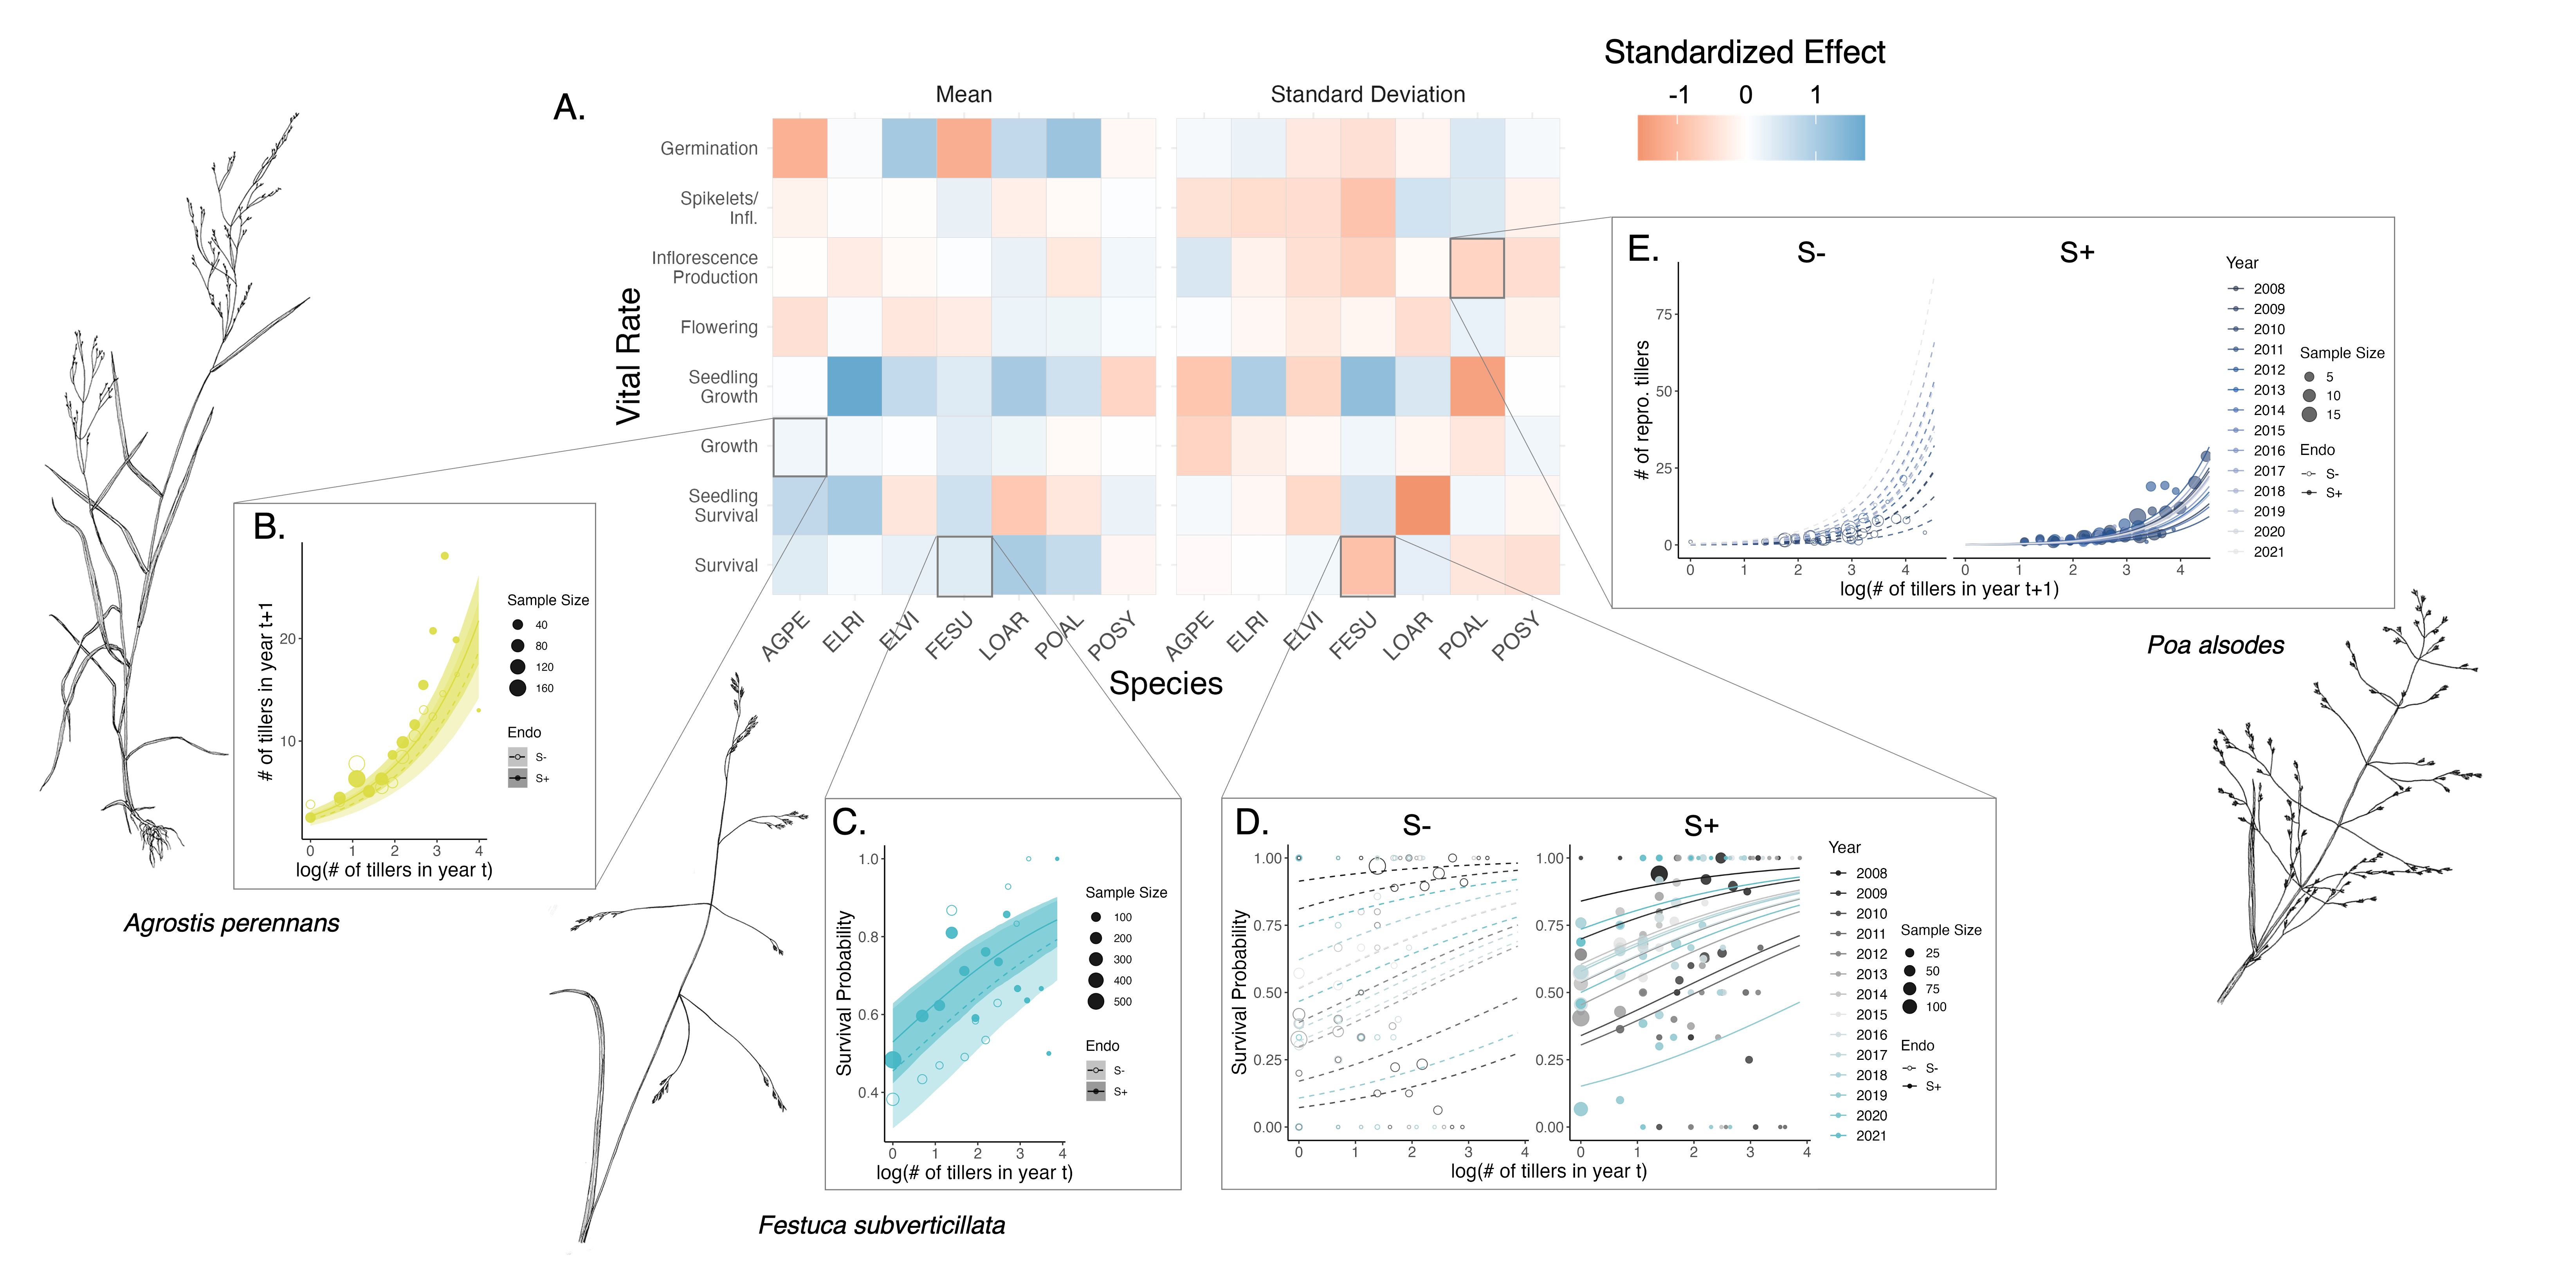
\includegraphics[width=\linewidth]{StochDemo_fig1.png}
\end{figure}
\noindent {\bf Fig. 1.} \textbf{Effects of endophyte symbiosis on host vital rates.} (A) Shading represents the mean standardized effect size of endophytes on mean and and variance of host vital rates (blue indicates a positive effect of symbiosis and blue indicates a negative effect on mean or standard deviation ). (B)\emph{A. perennans} experiences an increase in mean growth due to endophytes and \emph{F. subverticillata}experiences  (C) an increased mean and a (D) reduction in interannual variance in survival. (D) \emph{P. alsodes} experiences reduced variance in fertility.
\newpage

\begin{figure}
	\centering
	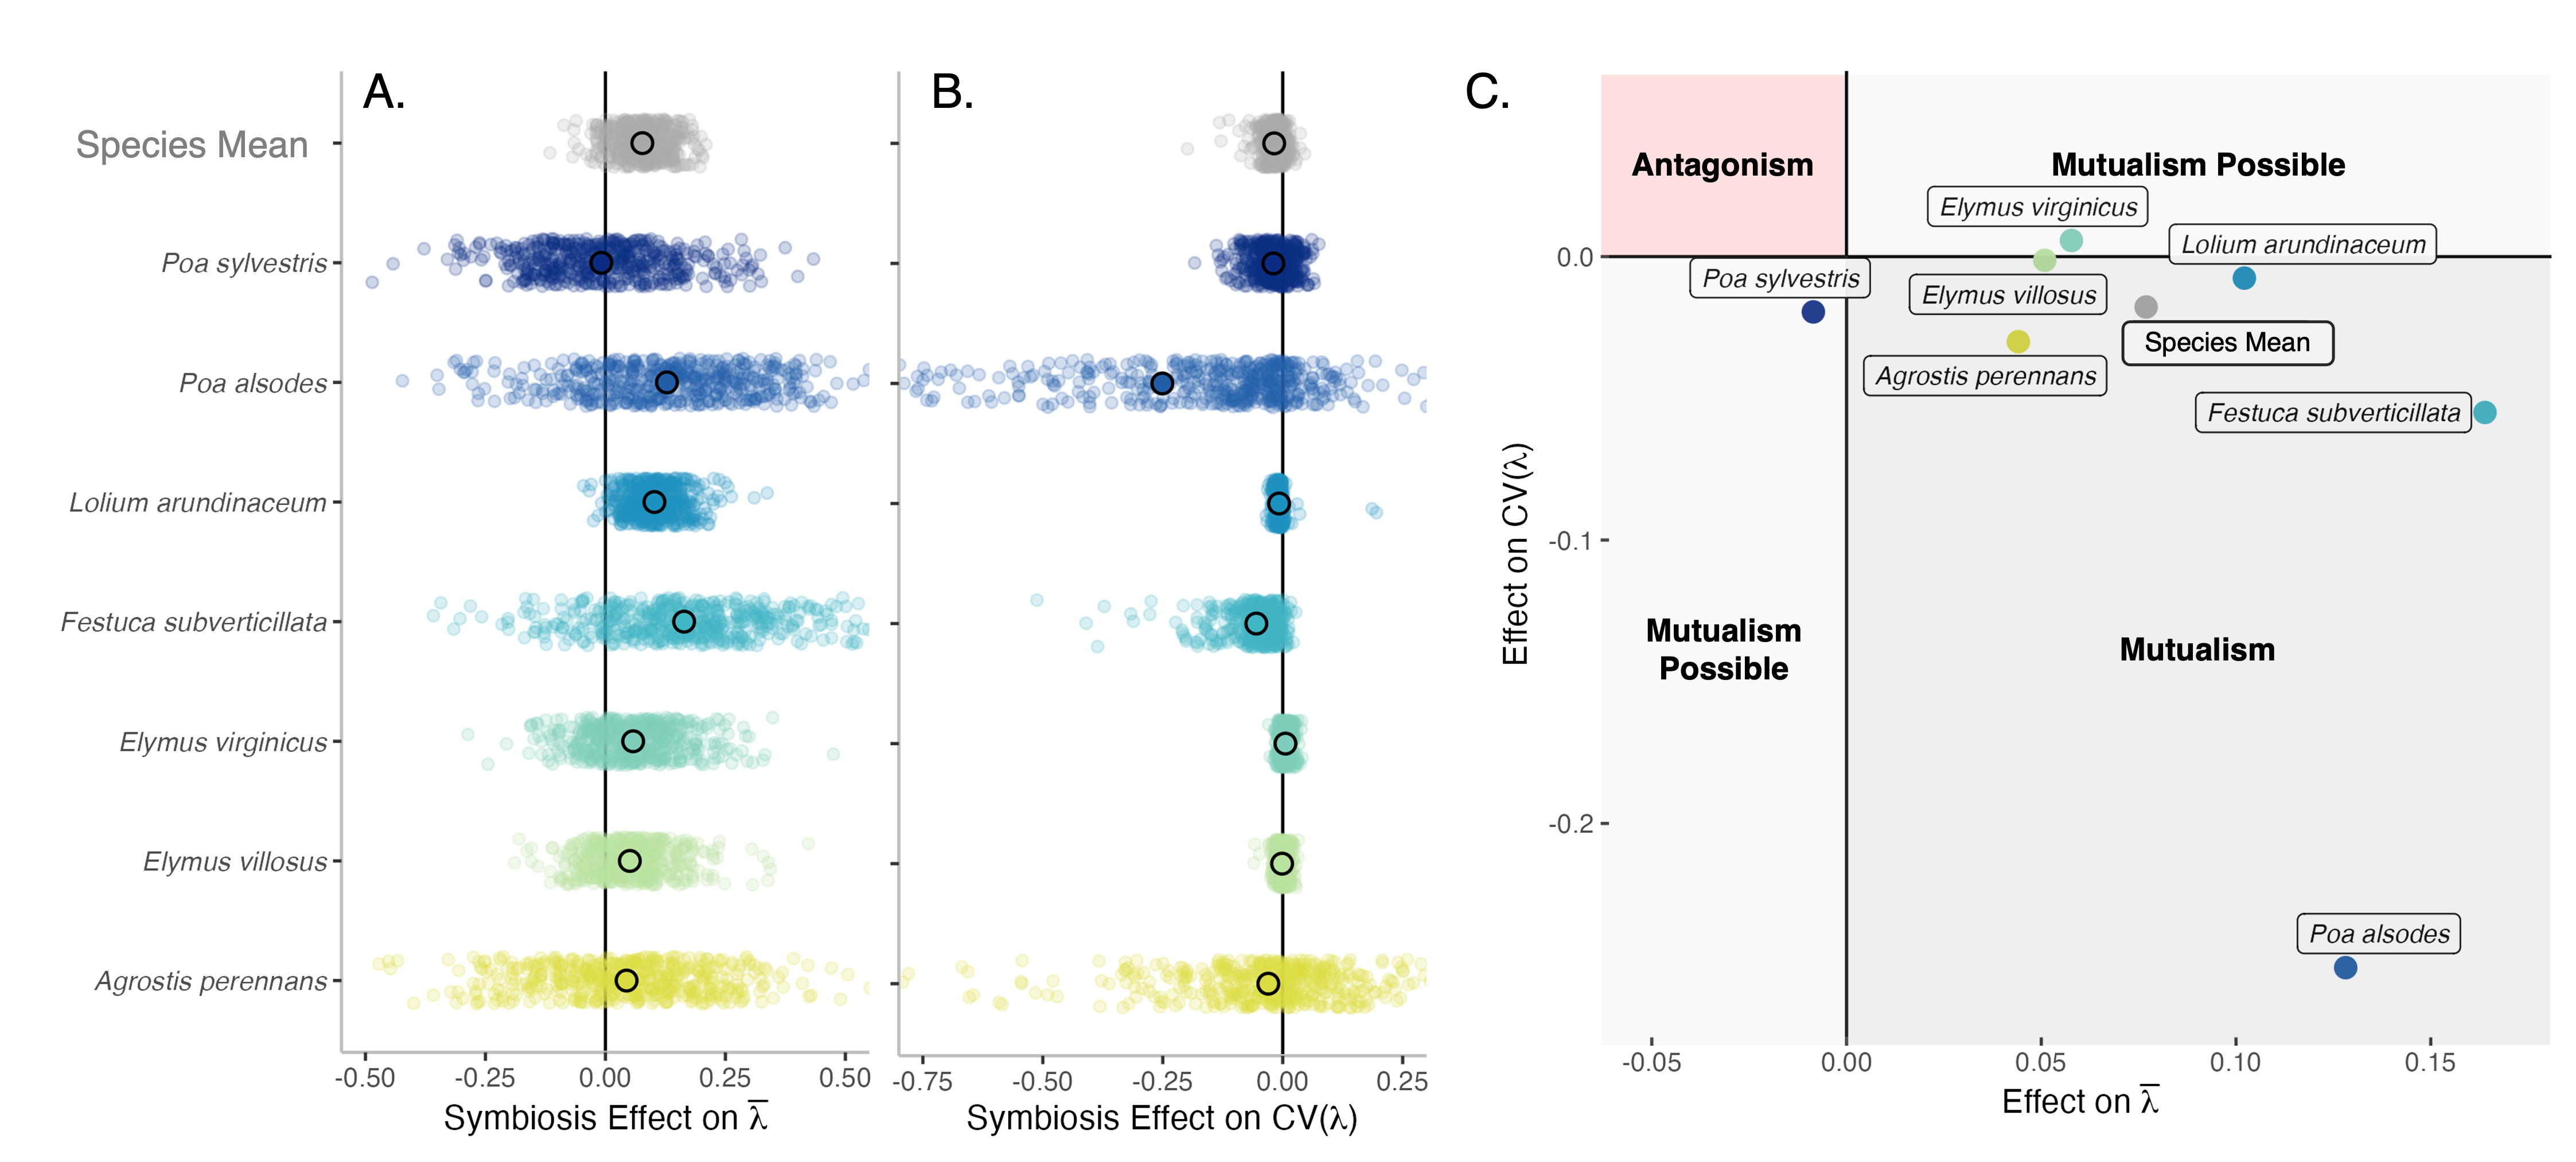
\includegraphics[width=\linewidth]{StochDemo_fig2.png}
\end{figure}
\noindent {\bf Fig. 2.} \textbf{Mean and variance-buffering effects on population growth rates.} Black circles indicate the average effect of endophytes along with 500 posterior draws (smaller colored circles) on the (A) mean and (B) coefficient of variation in population growth rates $\lambda$ for each host species. (C) For all hosts, endophyte either reduce variance, increase the mean, or both, and consequently when considering stochastic environments, the interactions are always at least potentially mutualistic.
\newpage

\begin{figure}
	\centering
	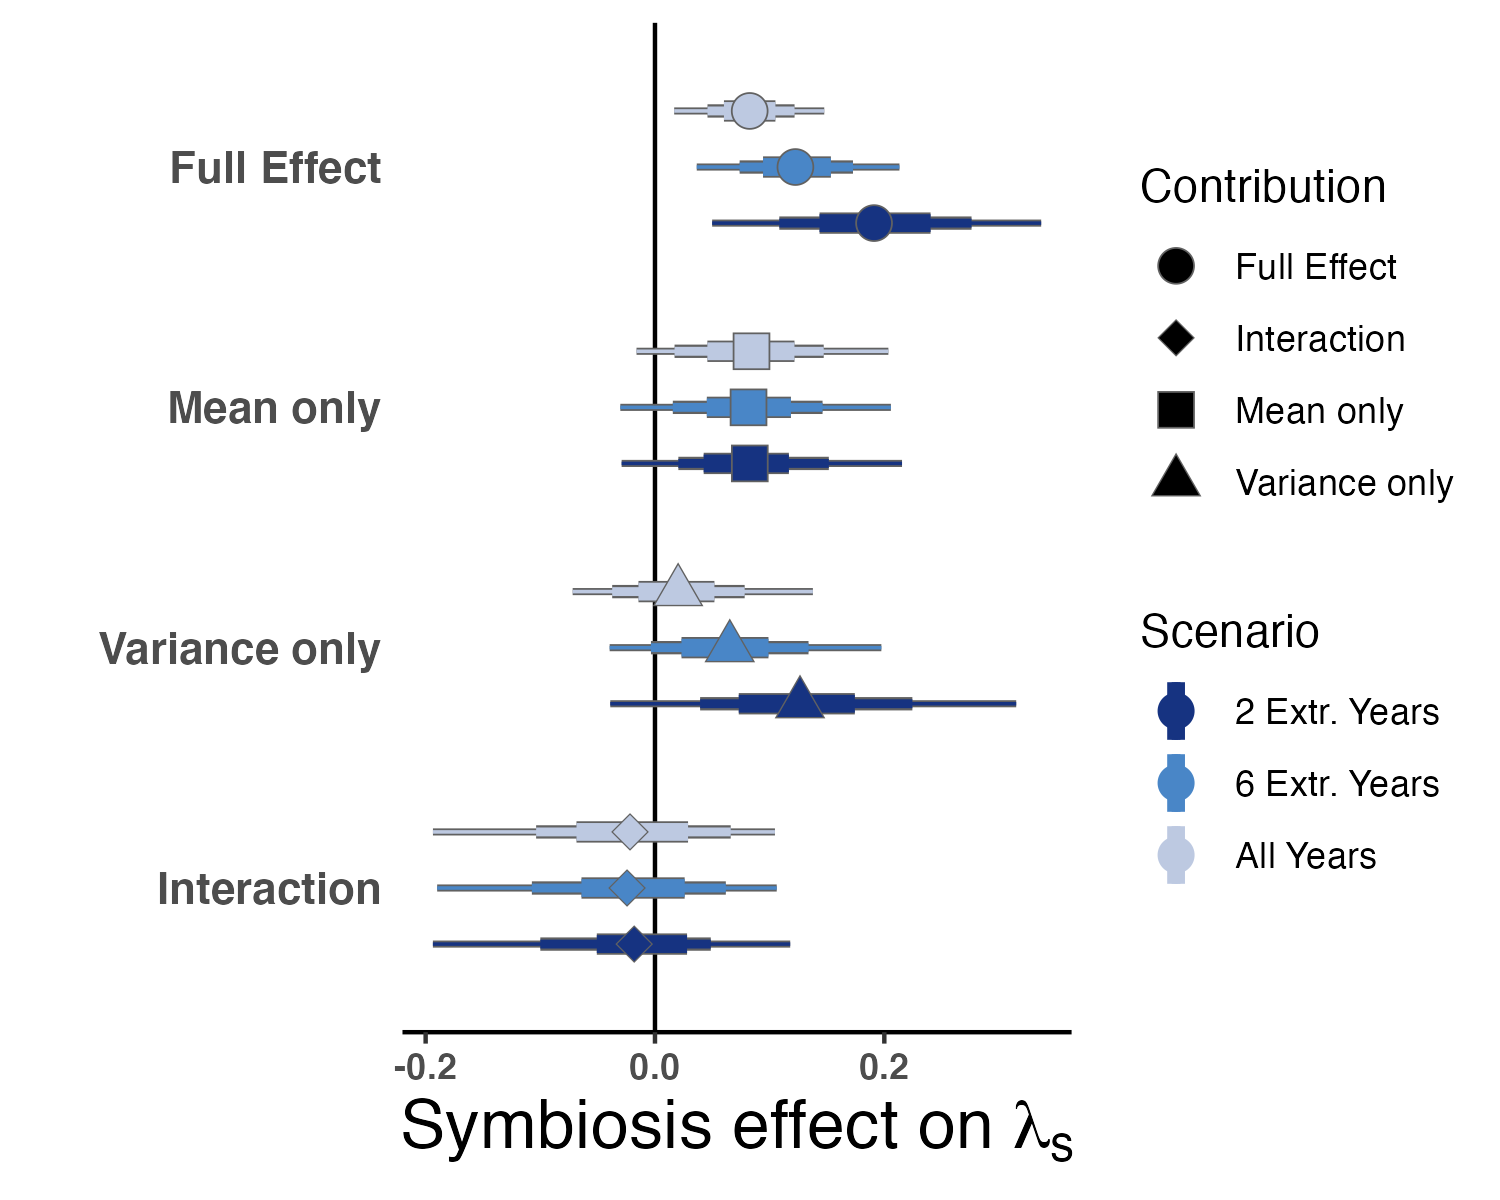
\includegraphics[width=.8\linewidth]{StochDemo_fig3.png}
\end{figure}
\noindent {\bf Fig. 3.} \textbf{Endophyte contributions to stochastic growth rates under observed and elevated variance.} The total effect of endophyte symbiosis comes from mean benefits and variance buffering as well as the interaction between mean and variance effects. Shapes indicate the posterior mean of each contribution, along with bars for the 50, 75 and 90 \% credible intervals.  The total effect of the symbiosis (circles) becomes more mutualistic under scenarios of increased variance (represented by color intensity). Contributions from mean effects (squares) remain constant while variance buffering effects (triangles) increase. A negative contribution from the mean-variance interaction makes sense in light of Eqn. 1, indicates that the variance penalty to stochastic growth depends on the mean value of annual growth rates such that variance is more detrimental for populations with low average growth rates.
\newpage


\begin{figure}
	\centering
	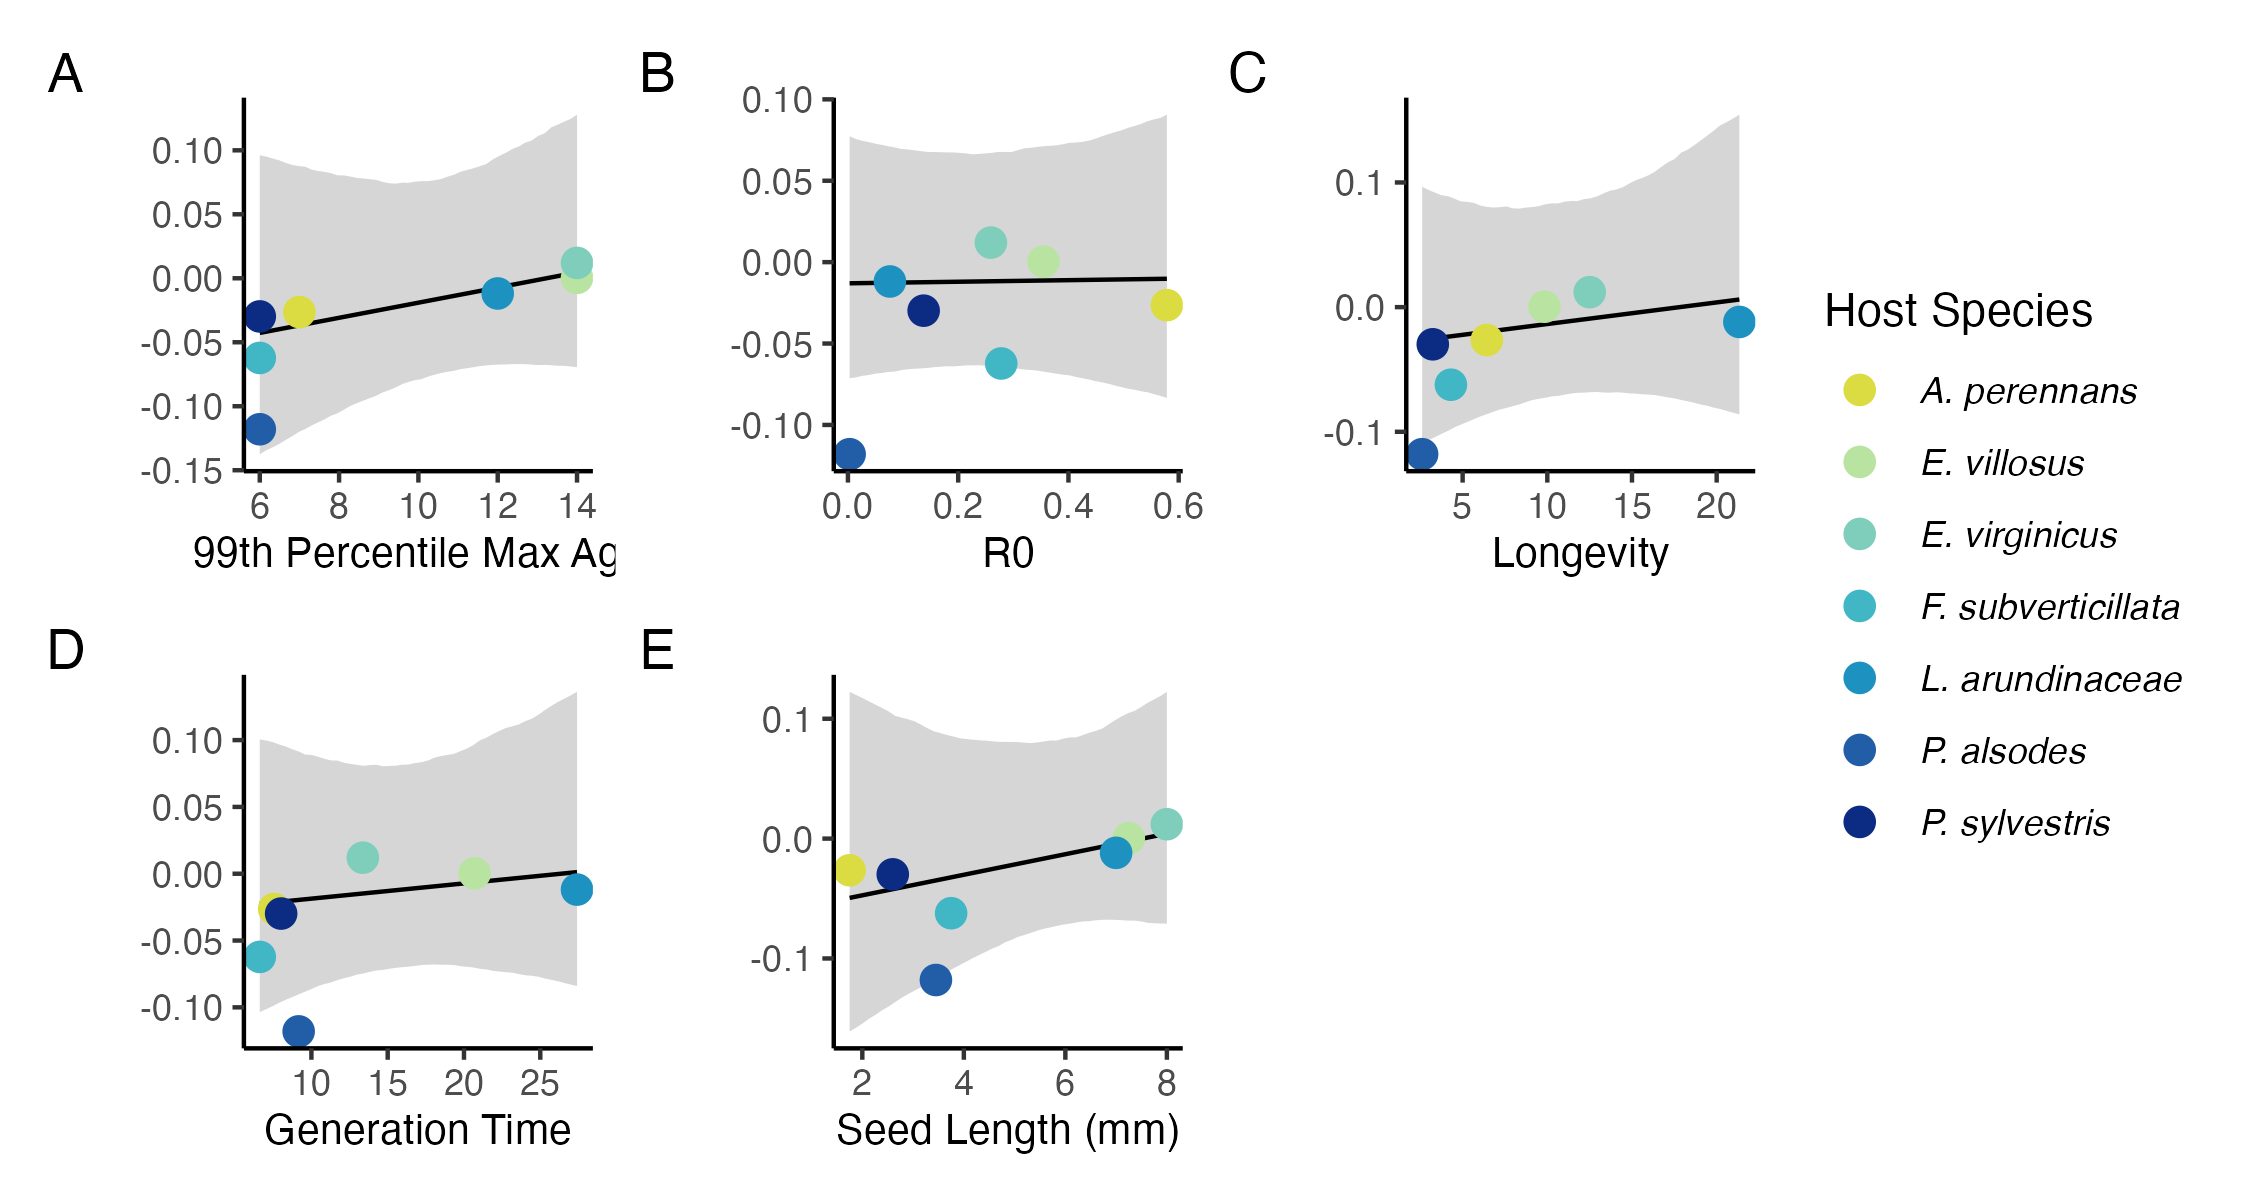
\includegraphics[width=\linewidth]{StochDemo_fig4.png}
\end{figure}
\noindent {\bf Fig. 4.} \textbf{Host species with faster life history traits experience stronger effects of symbiont-mediated variance buffering.} Linear regressions between life history traits describing the fast-slow life history continuum ((A) Maximum age observed during long term censuses; (B) 99th percentile maximum age during demographic censuses; (C) Net reproductive rate; (D) Longevity; (E) Mean life expectancy; (F) Generation time; (G) Seed size; (H) Rate of imperfect transmission) and the effect of endophyte symbiosis on the coefficent of variation in population growth rate ($\lambda$). Each panel shows the fitted mean relationship (line) along with with the 90\% credible interval.
\newpage


\begin{figure}
	\centering
	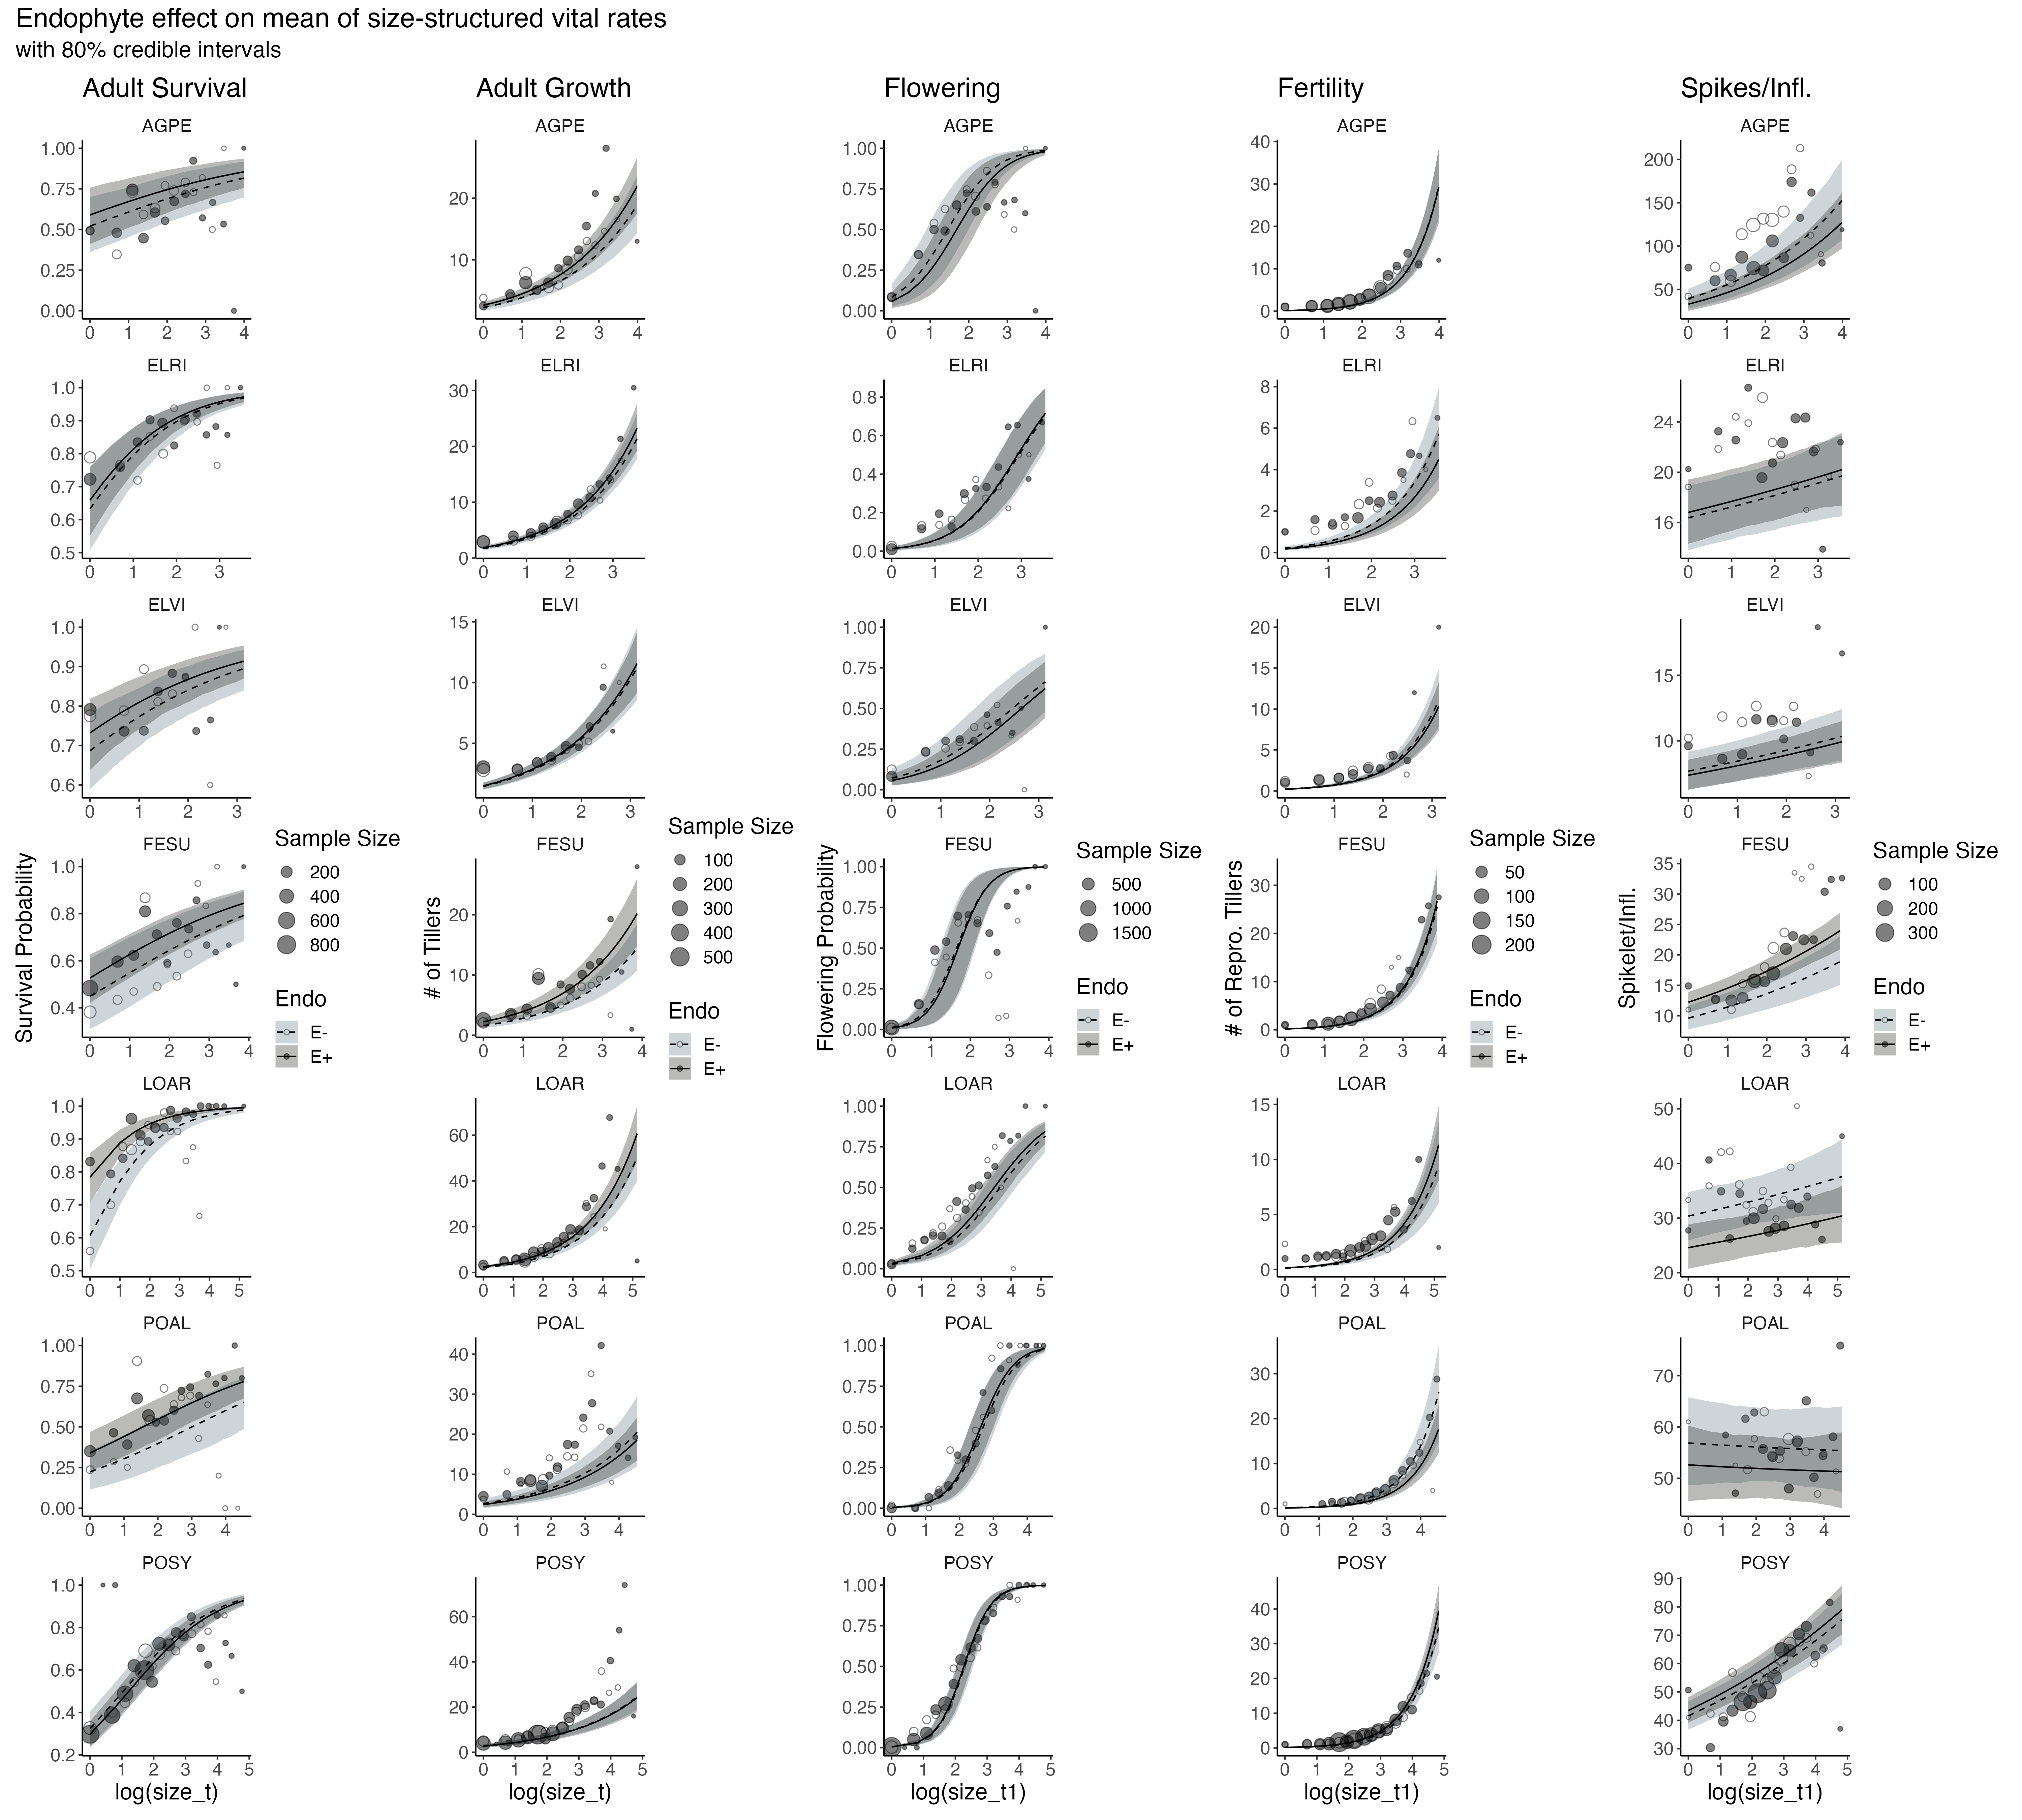
\includegraphics[width=\linewidth]{figS1_meaneffect_fitplot.png}
\end{figure}
\noindent {\bf Fig. S1.} \textbf{Effect of endophyte partnership on the mean value of size dependent vital rates.} Dashed line represents the expected model value along with data binned by size shown as open circles for symbiotic (E+) plants , while the solid line and filled circles represent symbiont-free (E-) plants. Each is shown along with an 80\% credible interval (darker shading: E-; lighter shading: E+).
\newpage

\begin{figure}
	\centering
	\includegraphics[width=\linewidth]{figS2_vareffect_fitplot.png}
\end{figure}
\noindent {\bf Fig. S2.} \textbf{Effect of endophyte partnership on interannual variance of size dependent vital rates.} Dashed lines represent the expected model value colored by census year,  along with data binned by size shown as open circles for symbiotic (E+) plants, while the solid line and filled circles represent symbiont-free (E-) plants. Size of points reflects sample size.
\newpage

\begin{figure}
	\centering
	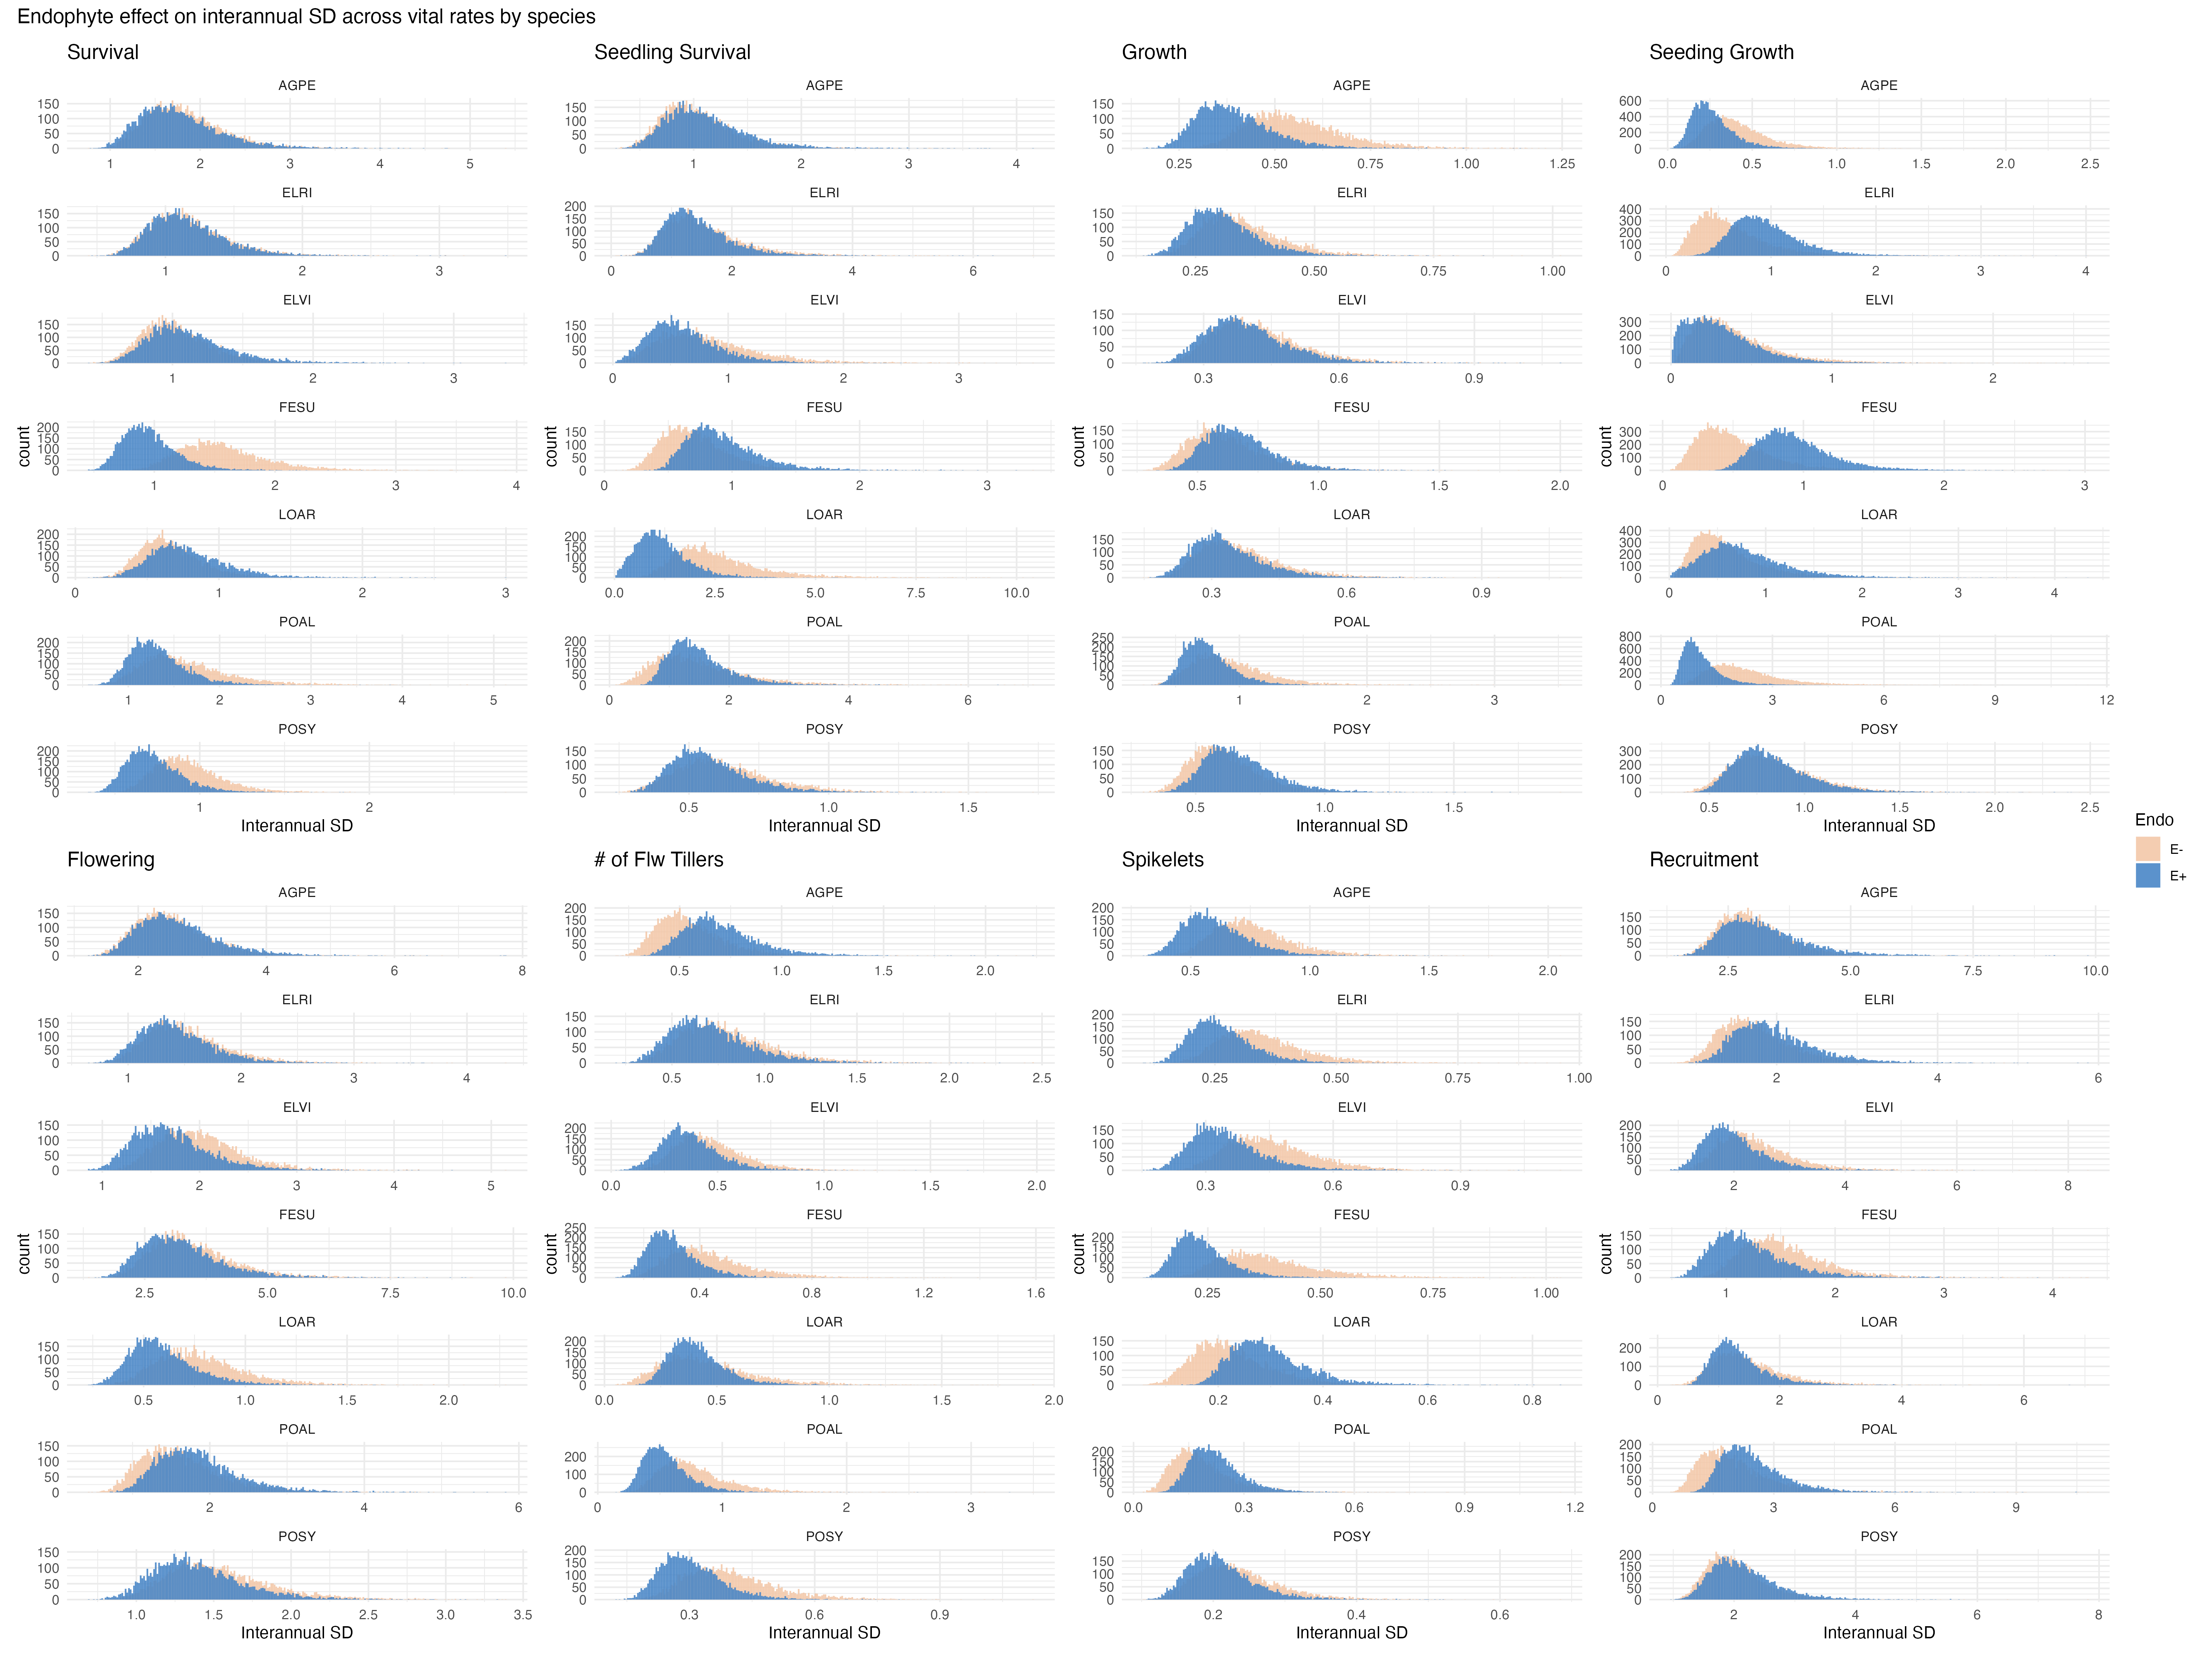
\includegraphics[width=\linewidth]{figS3_endo_sigmayear_histograms.png}
\end{figure}
\noindent {\bf Fig. S3.} \textbf{Posterior distributions of the standard deviations of interannual year effects.} Histograms include 7500 post-warmup MCMC samples for symbiotic (E+; blue) and symbiont-free (E-;tan) plants from fitted vital rate models.
\newpage

\begin{figure}
	\centering
	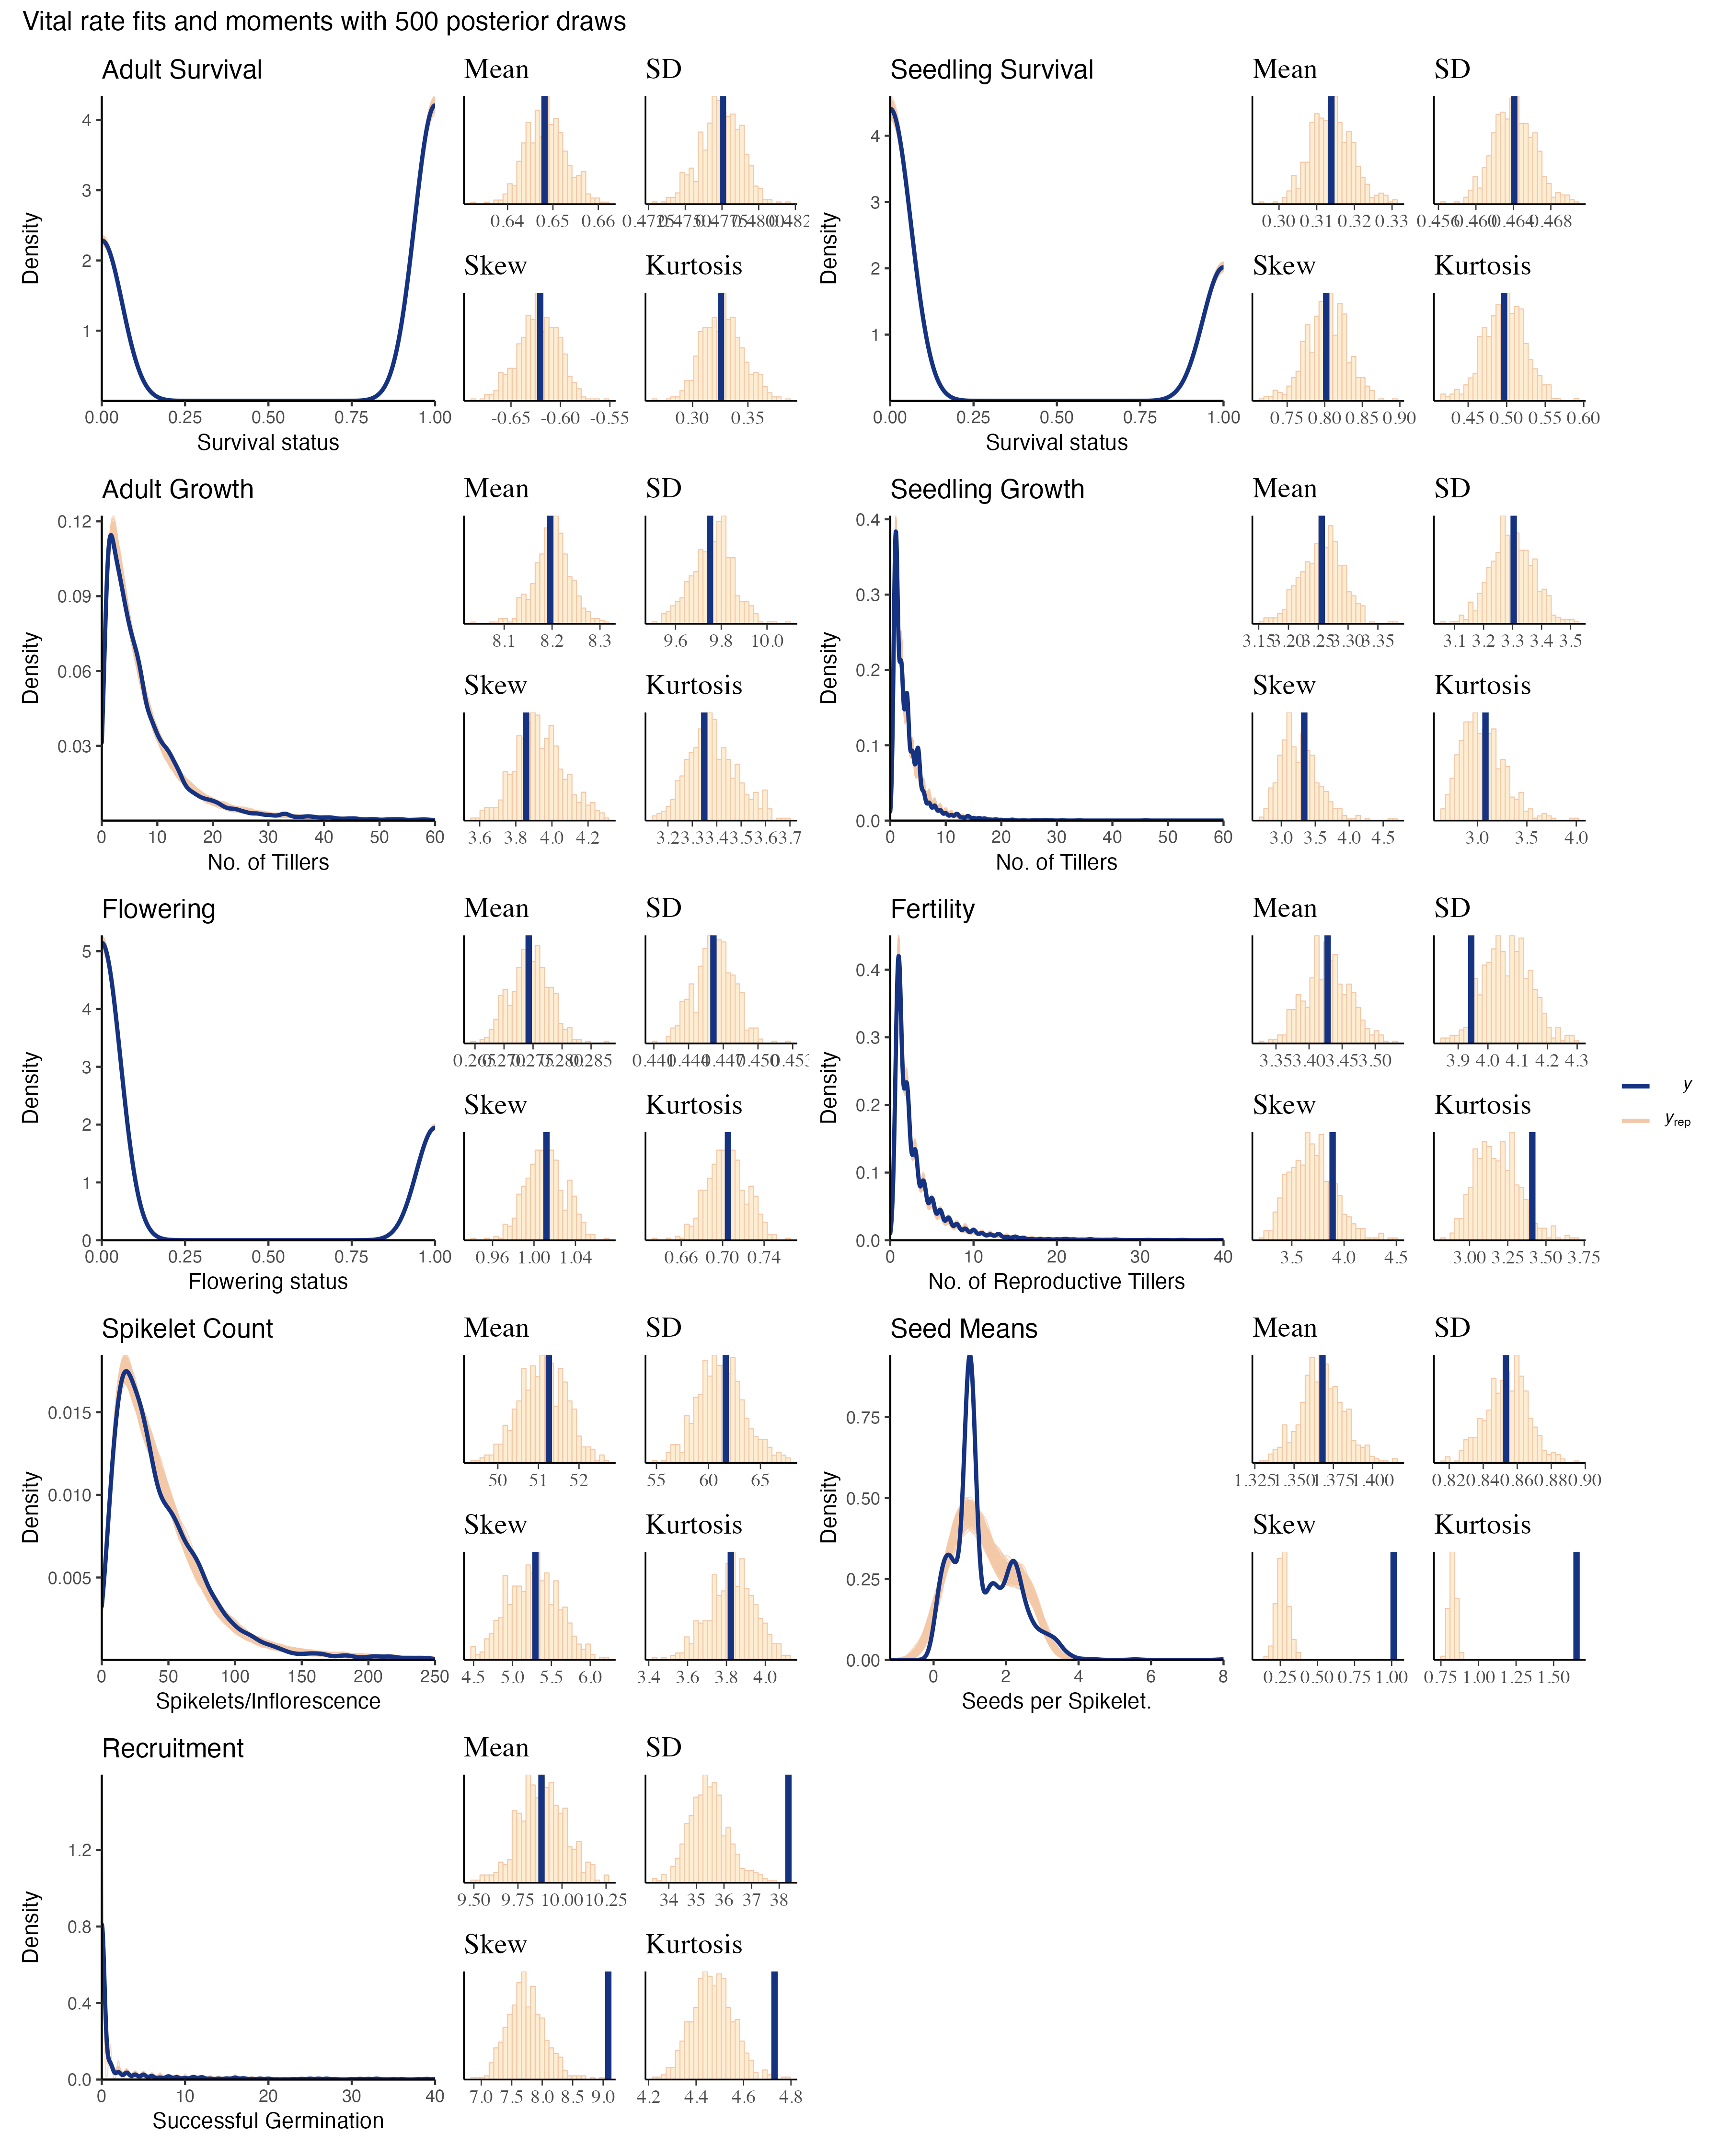
\includegraphics[width=.7\linewidth]{figS4_fitsandmoments_plot.png}
\end{figure}
\noindent {\bf Fig. S4.} \textbf{Posterior predictive check for statistical models of demographic vital rates.} Lines show density distributions of observed data (blue line) compared to data simulated from fitted models (tan lines) generated from 500 draws from posterior distributions of model parameters. Consistency between real simulated data indicates that fitted models describe the data well.
\newpage

\begin{figure}
	\centering
	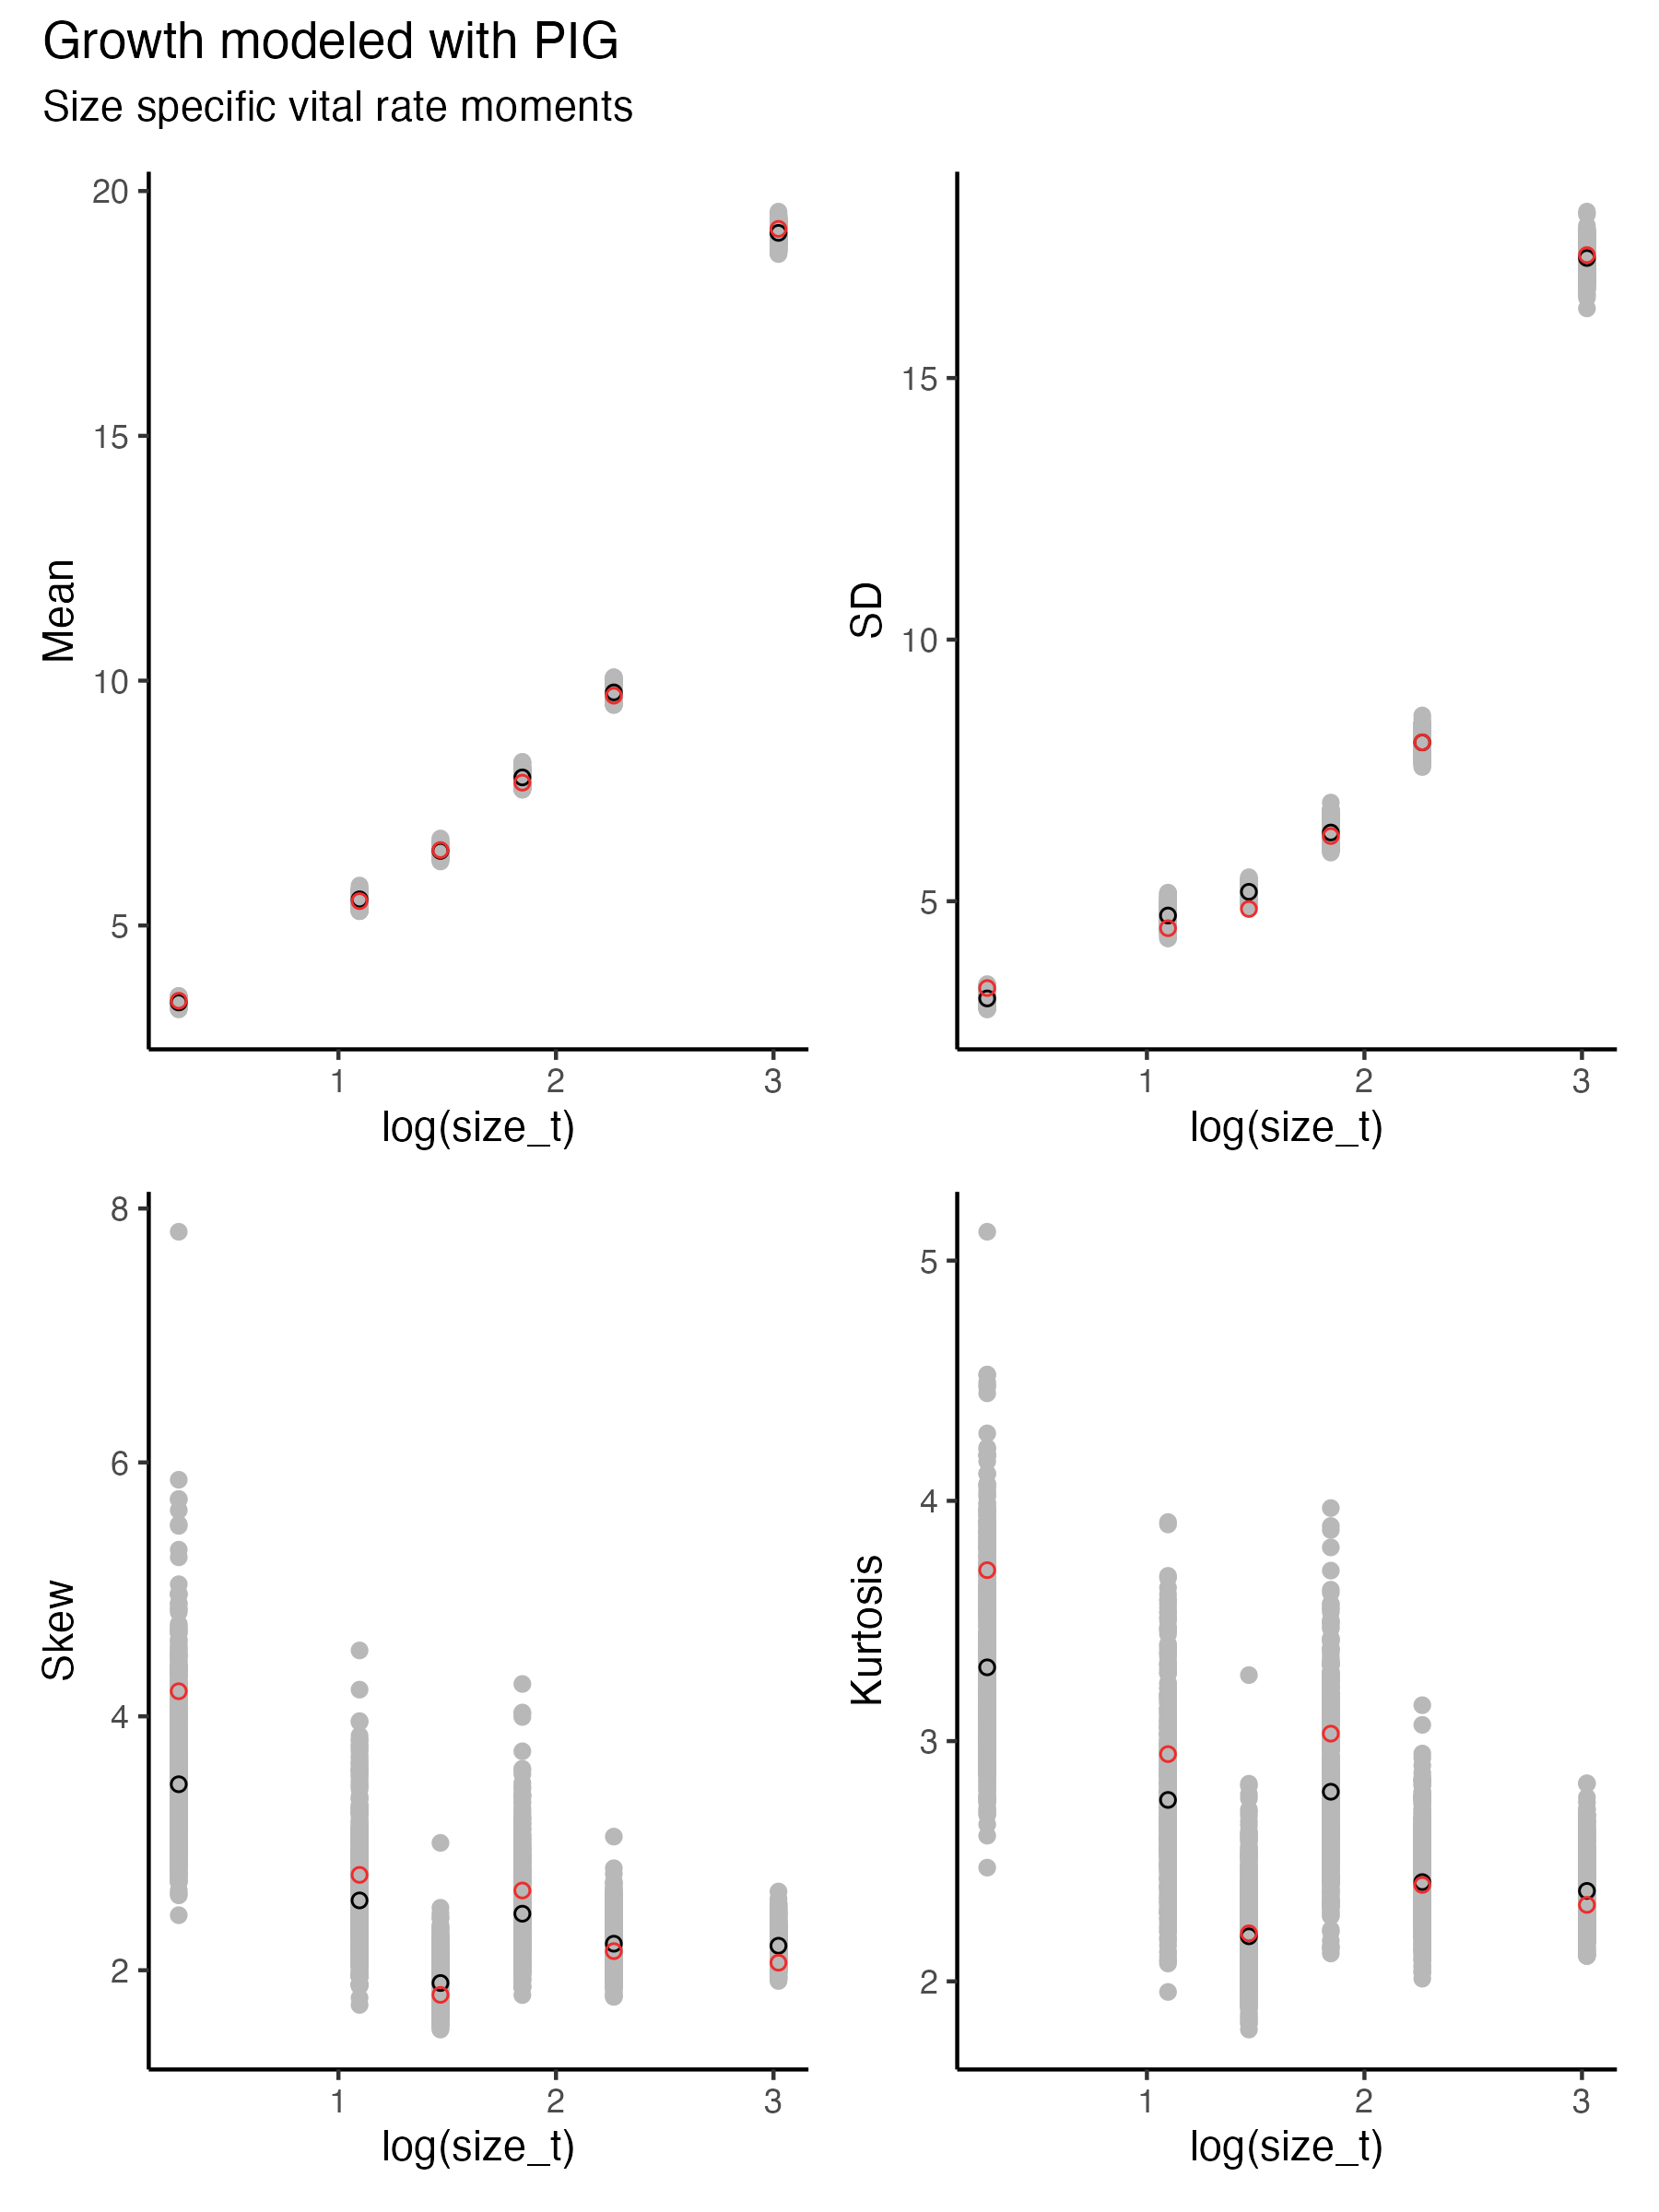
\includegraphics[width=.6\linewidth]{figS5_size_ppc_plot.png}
\end{figure}
\noindent {\bf Fig. S5.} \textbf{Posterior predictive check for mean and higher moments of the growth model across size.} Points show the value of statistical moments binned across size for the observed data (red circles) compared to the simulated datasets (grey circles) and the median of the simulated values (black circles) generated from 500 posterior draws from the fitted model. Consistency between real data and fitted valued across sizes indicates that the growth model is accurately capturing size dependence.
\newpage

\begin{figure}
	\centering
	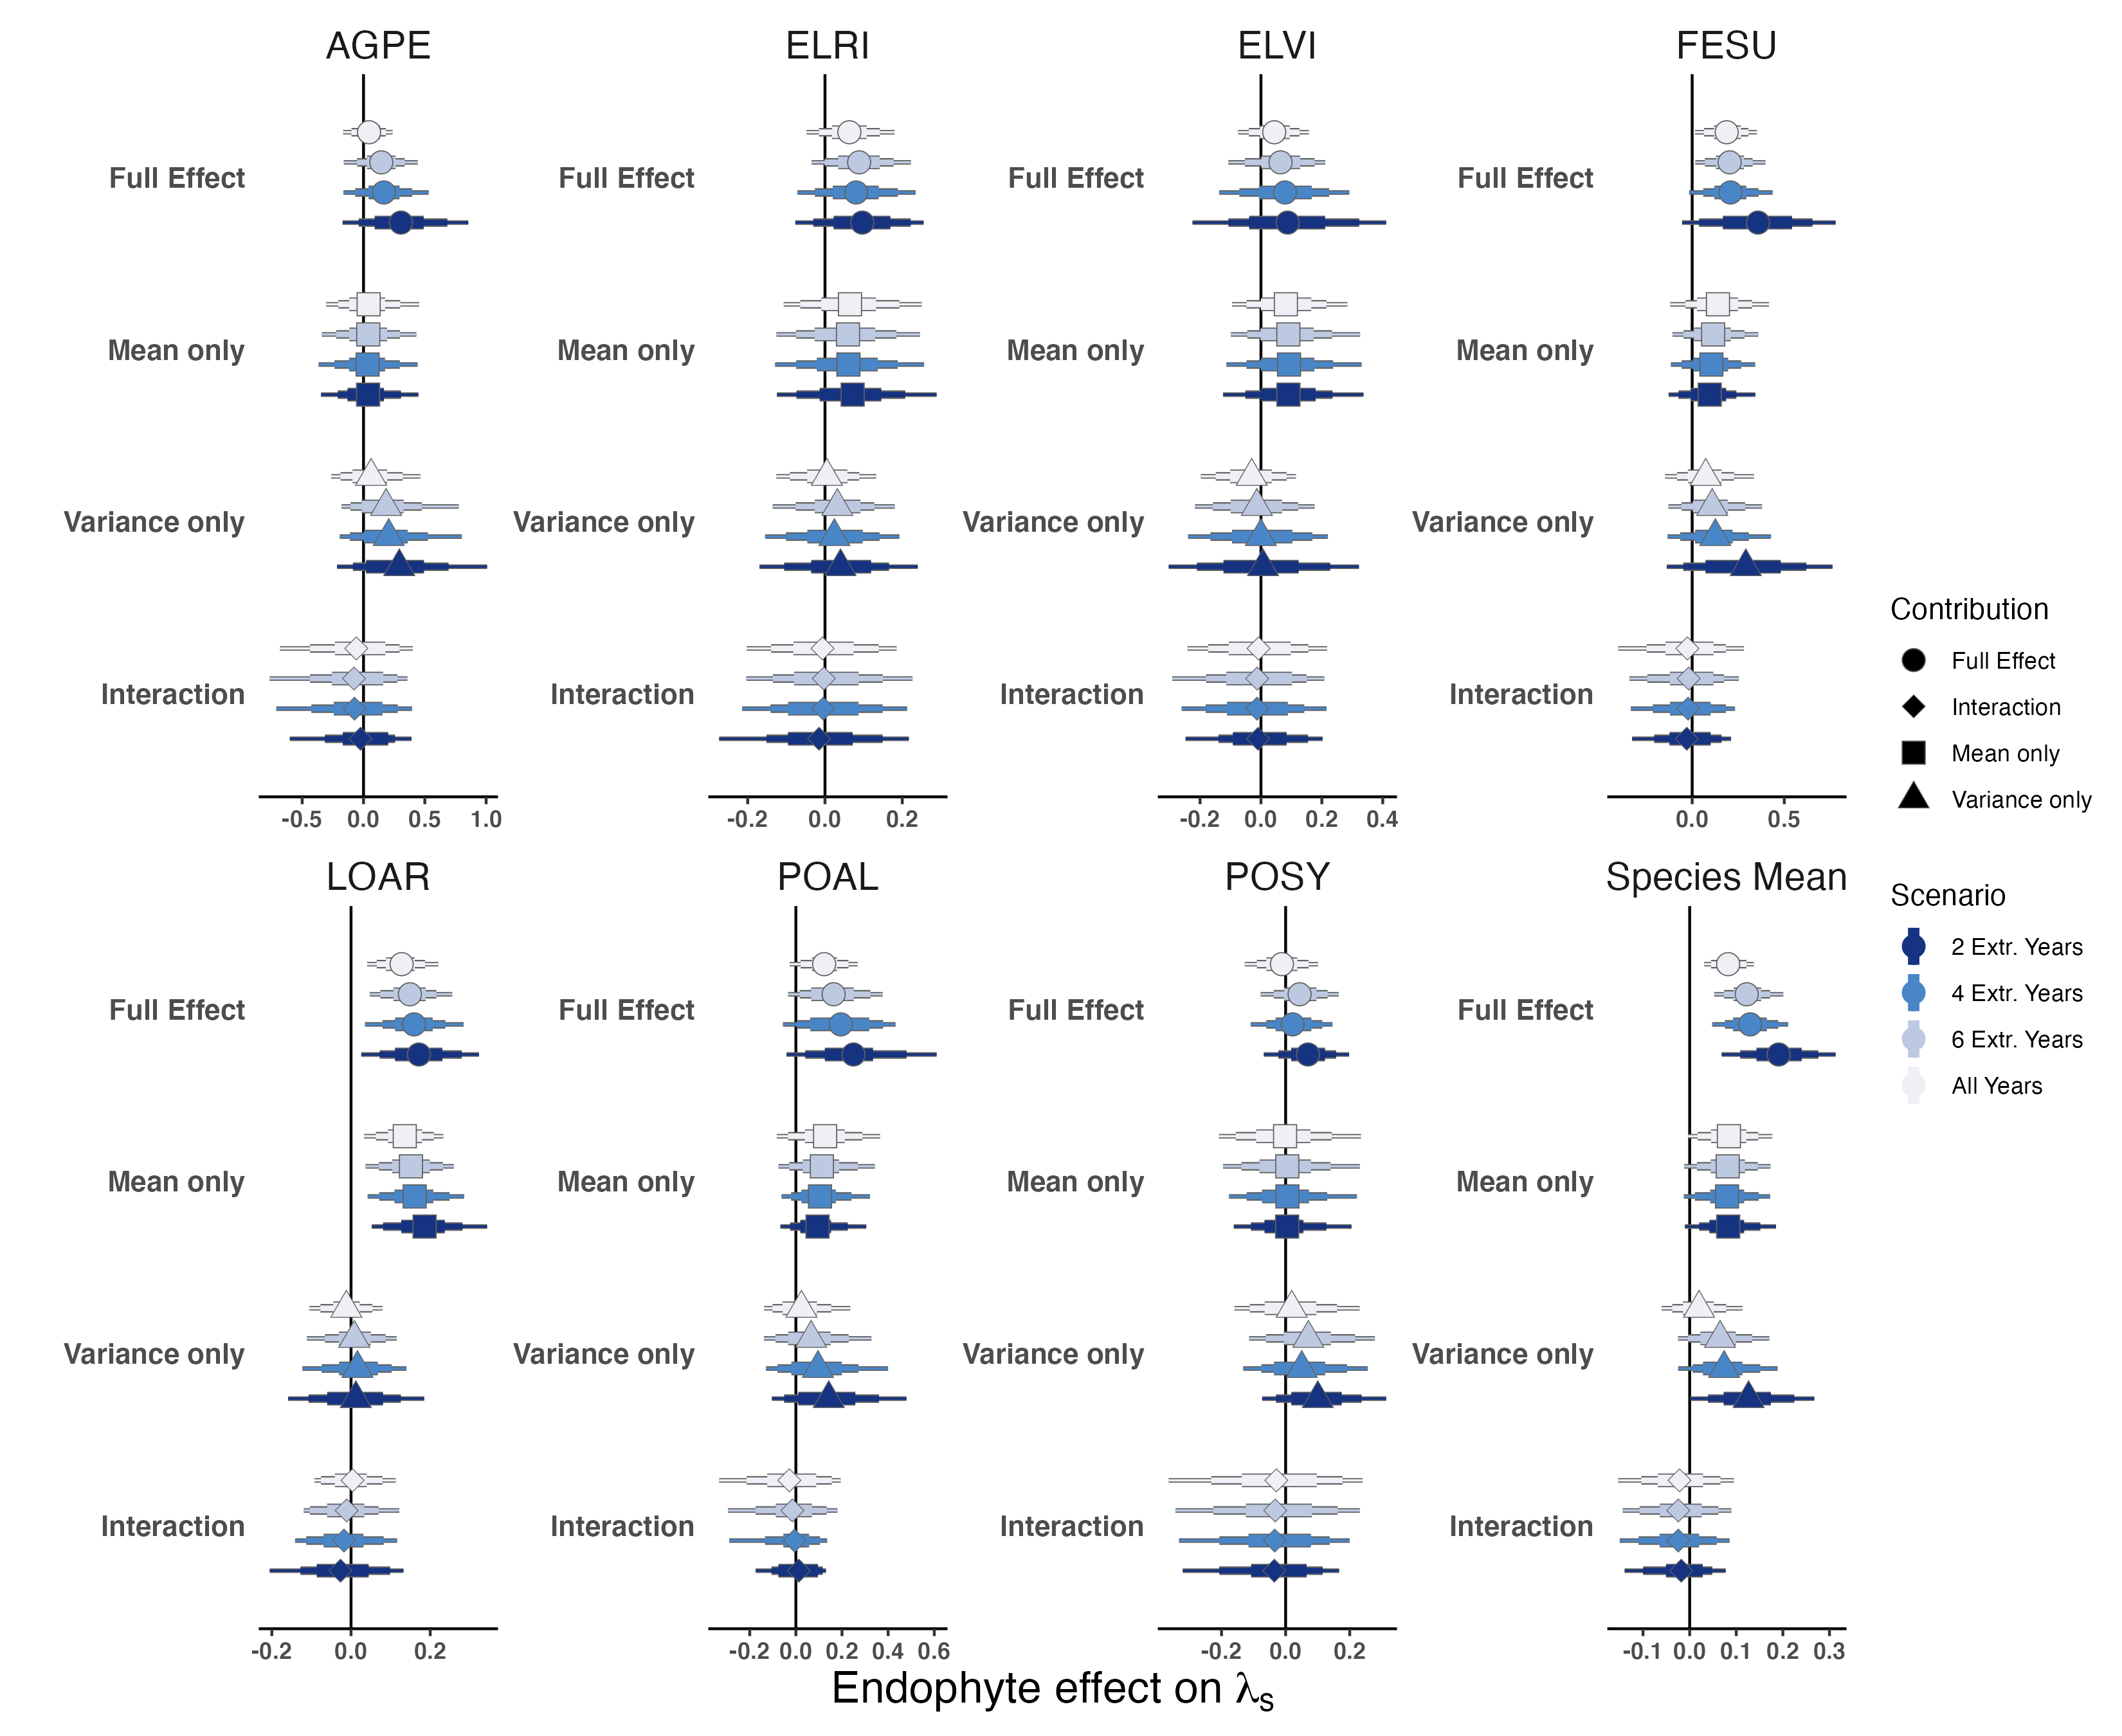
\includegraphics[width=\linewidth]{figS6_contributions_obs_plot.png}
\end{figure}
\noindent {\bf Fig. S6.} \textbf{Endophyte contributions to stochastic growth rates under observed and elevated variance across species.} The total effect of endophytes (circle) comes from mean benefits (square) and variance buffering (triangle) as well as the interaction between mean and variance effects (diamond). Shapes indicate the posterior mean of each contribution, along with bars for the 50, 75 and 90 \% credible intervals.  Under scenarios of increasing variance, represented by increasing color intensity, effects of variance buffering increase leading to a more mutualistic symbiosis.
\newpage

\begin{figure}
	\centering
	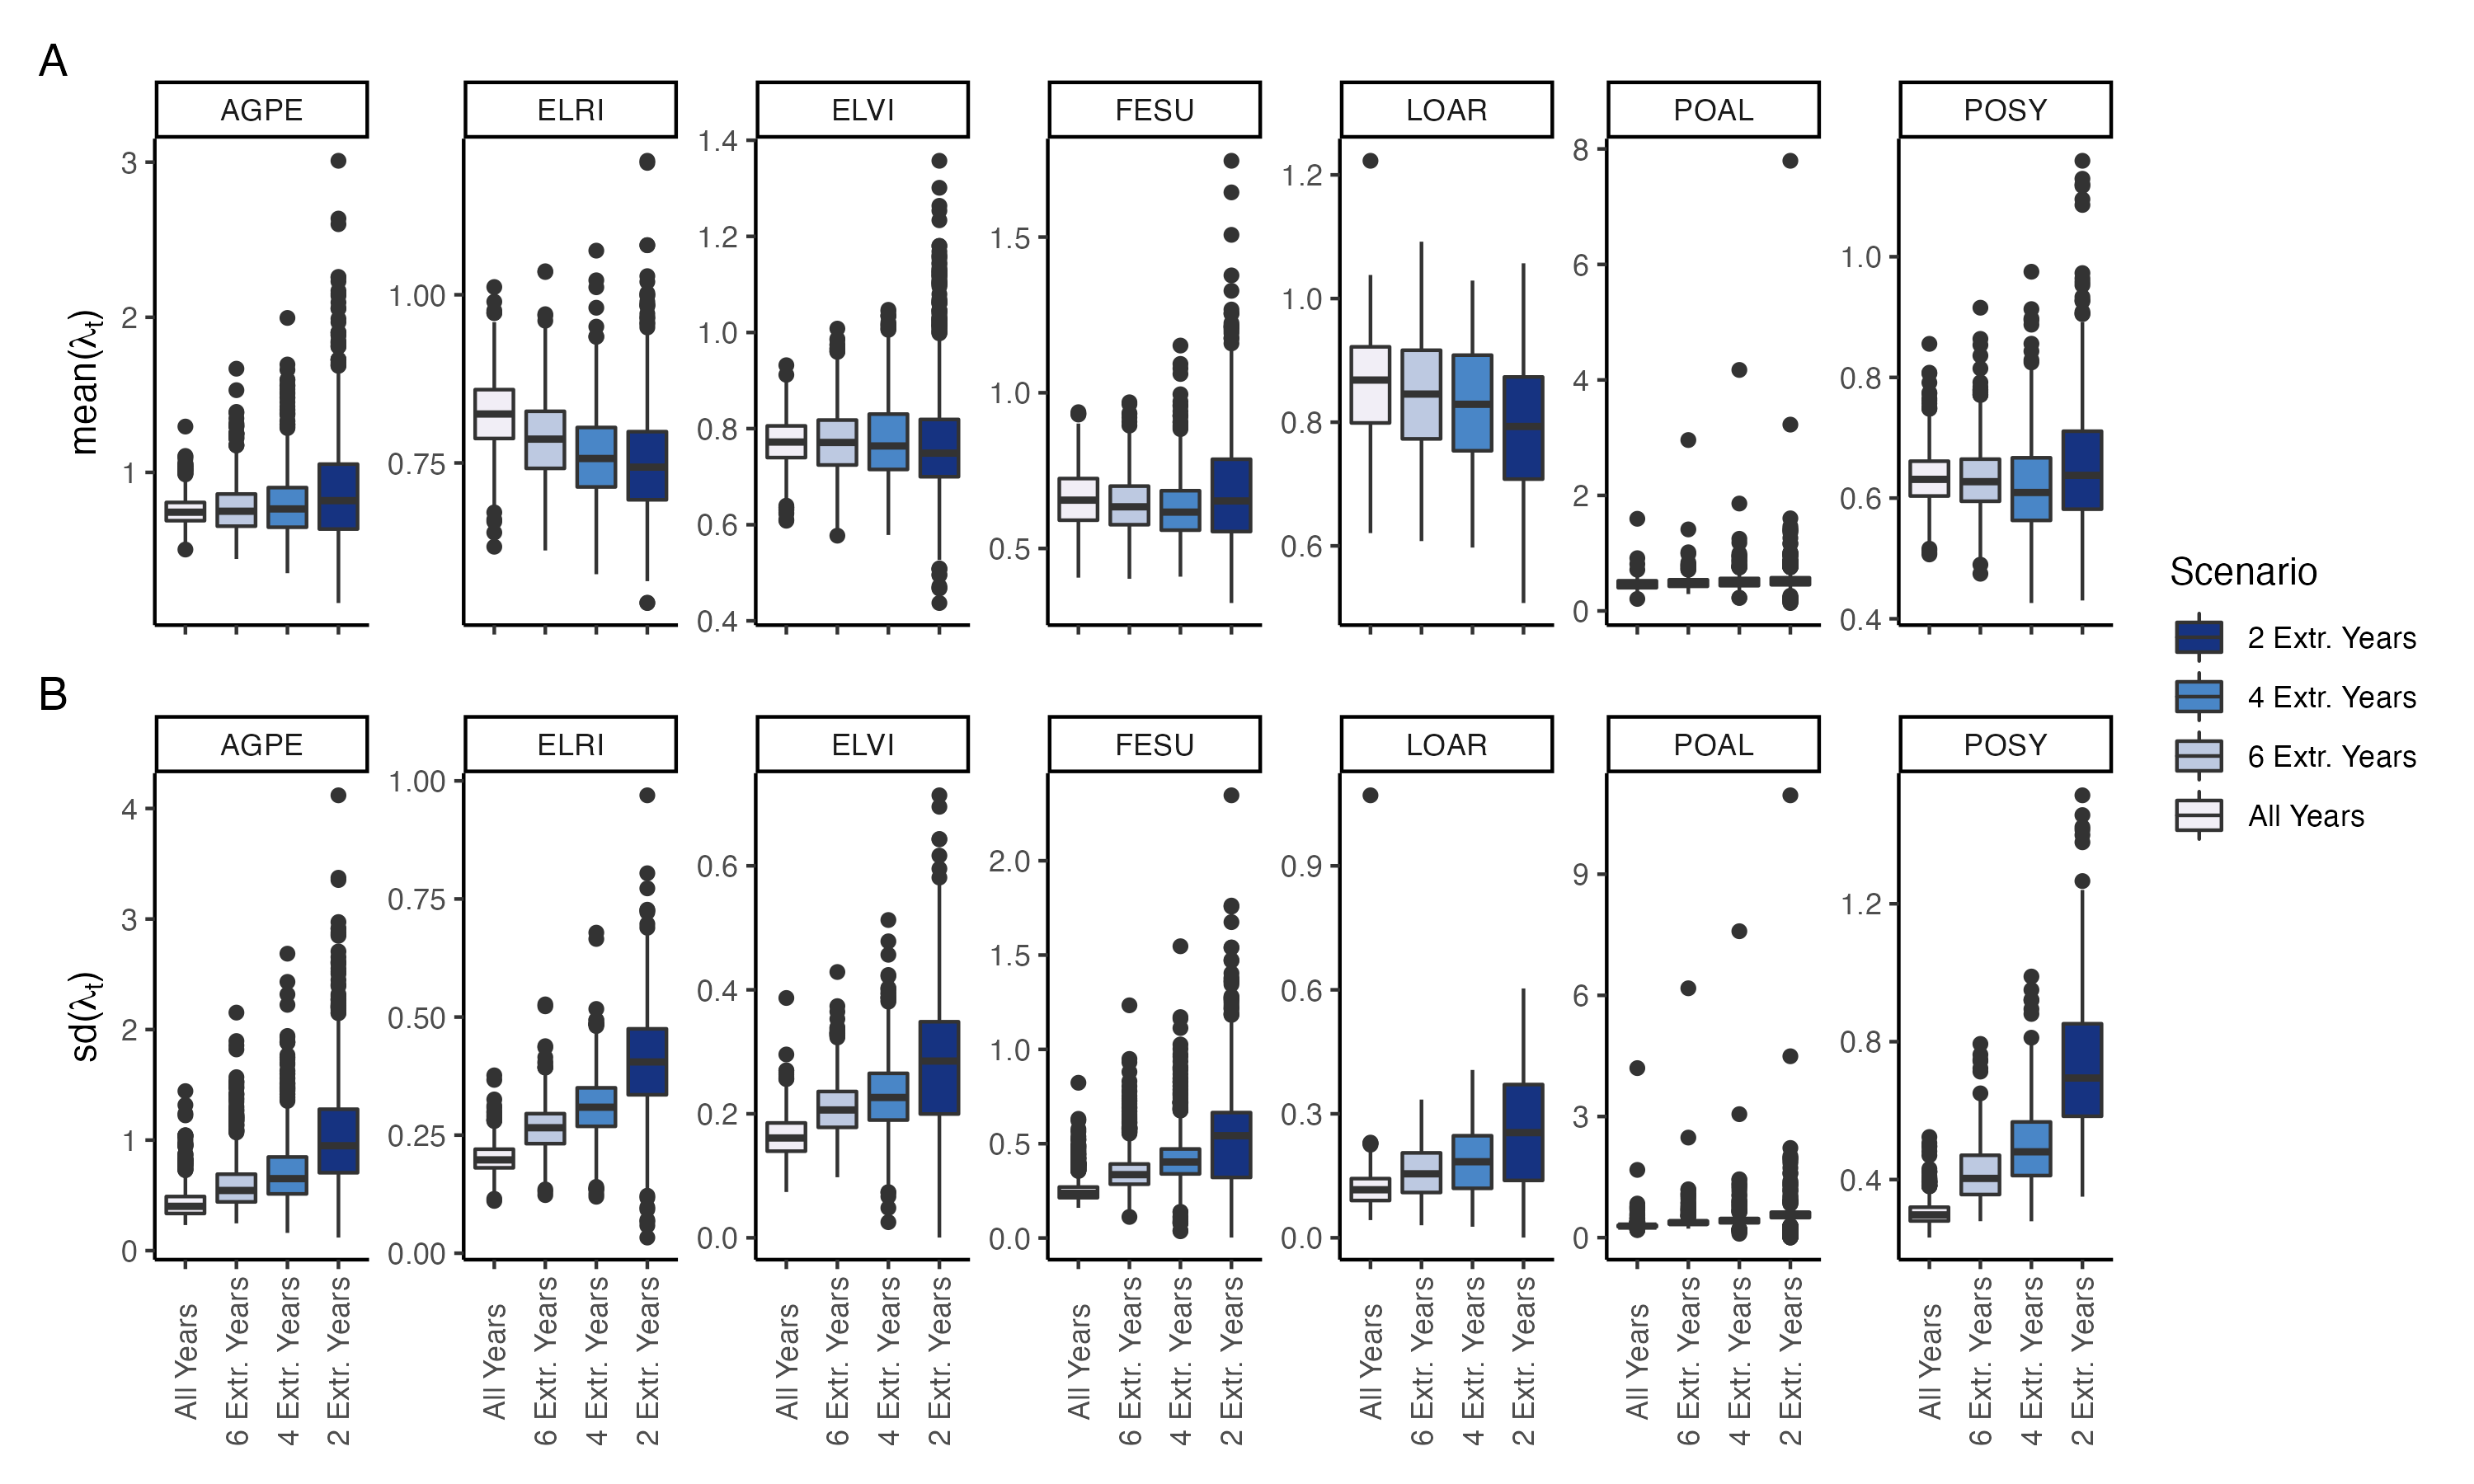
\includegraphics[width=\linewidth]{figS7_sim_boxplots.png}
\end{figure}
\noindent {\bf Fig. S7.} \textbf{(A) Mean and (B) standard deviation of annual growth rate values during simulation scenarios.} Each scenario selects from observed transition matrixes, increasing the variance by selecting either all observed years, or a set (6, 4, or 2 years) that have the highest and lowest growth rates for symbiont-free populations.
\newpage


\begin{figure}
	\centering
	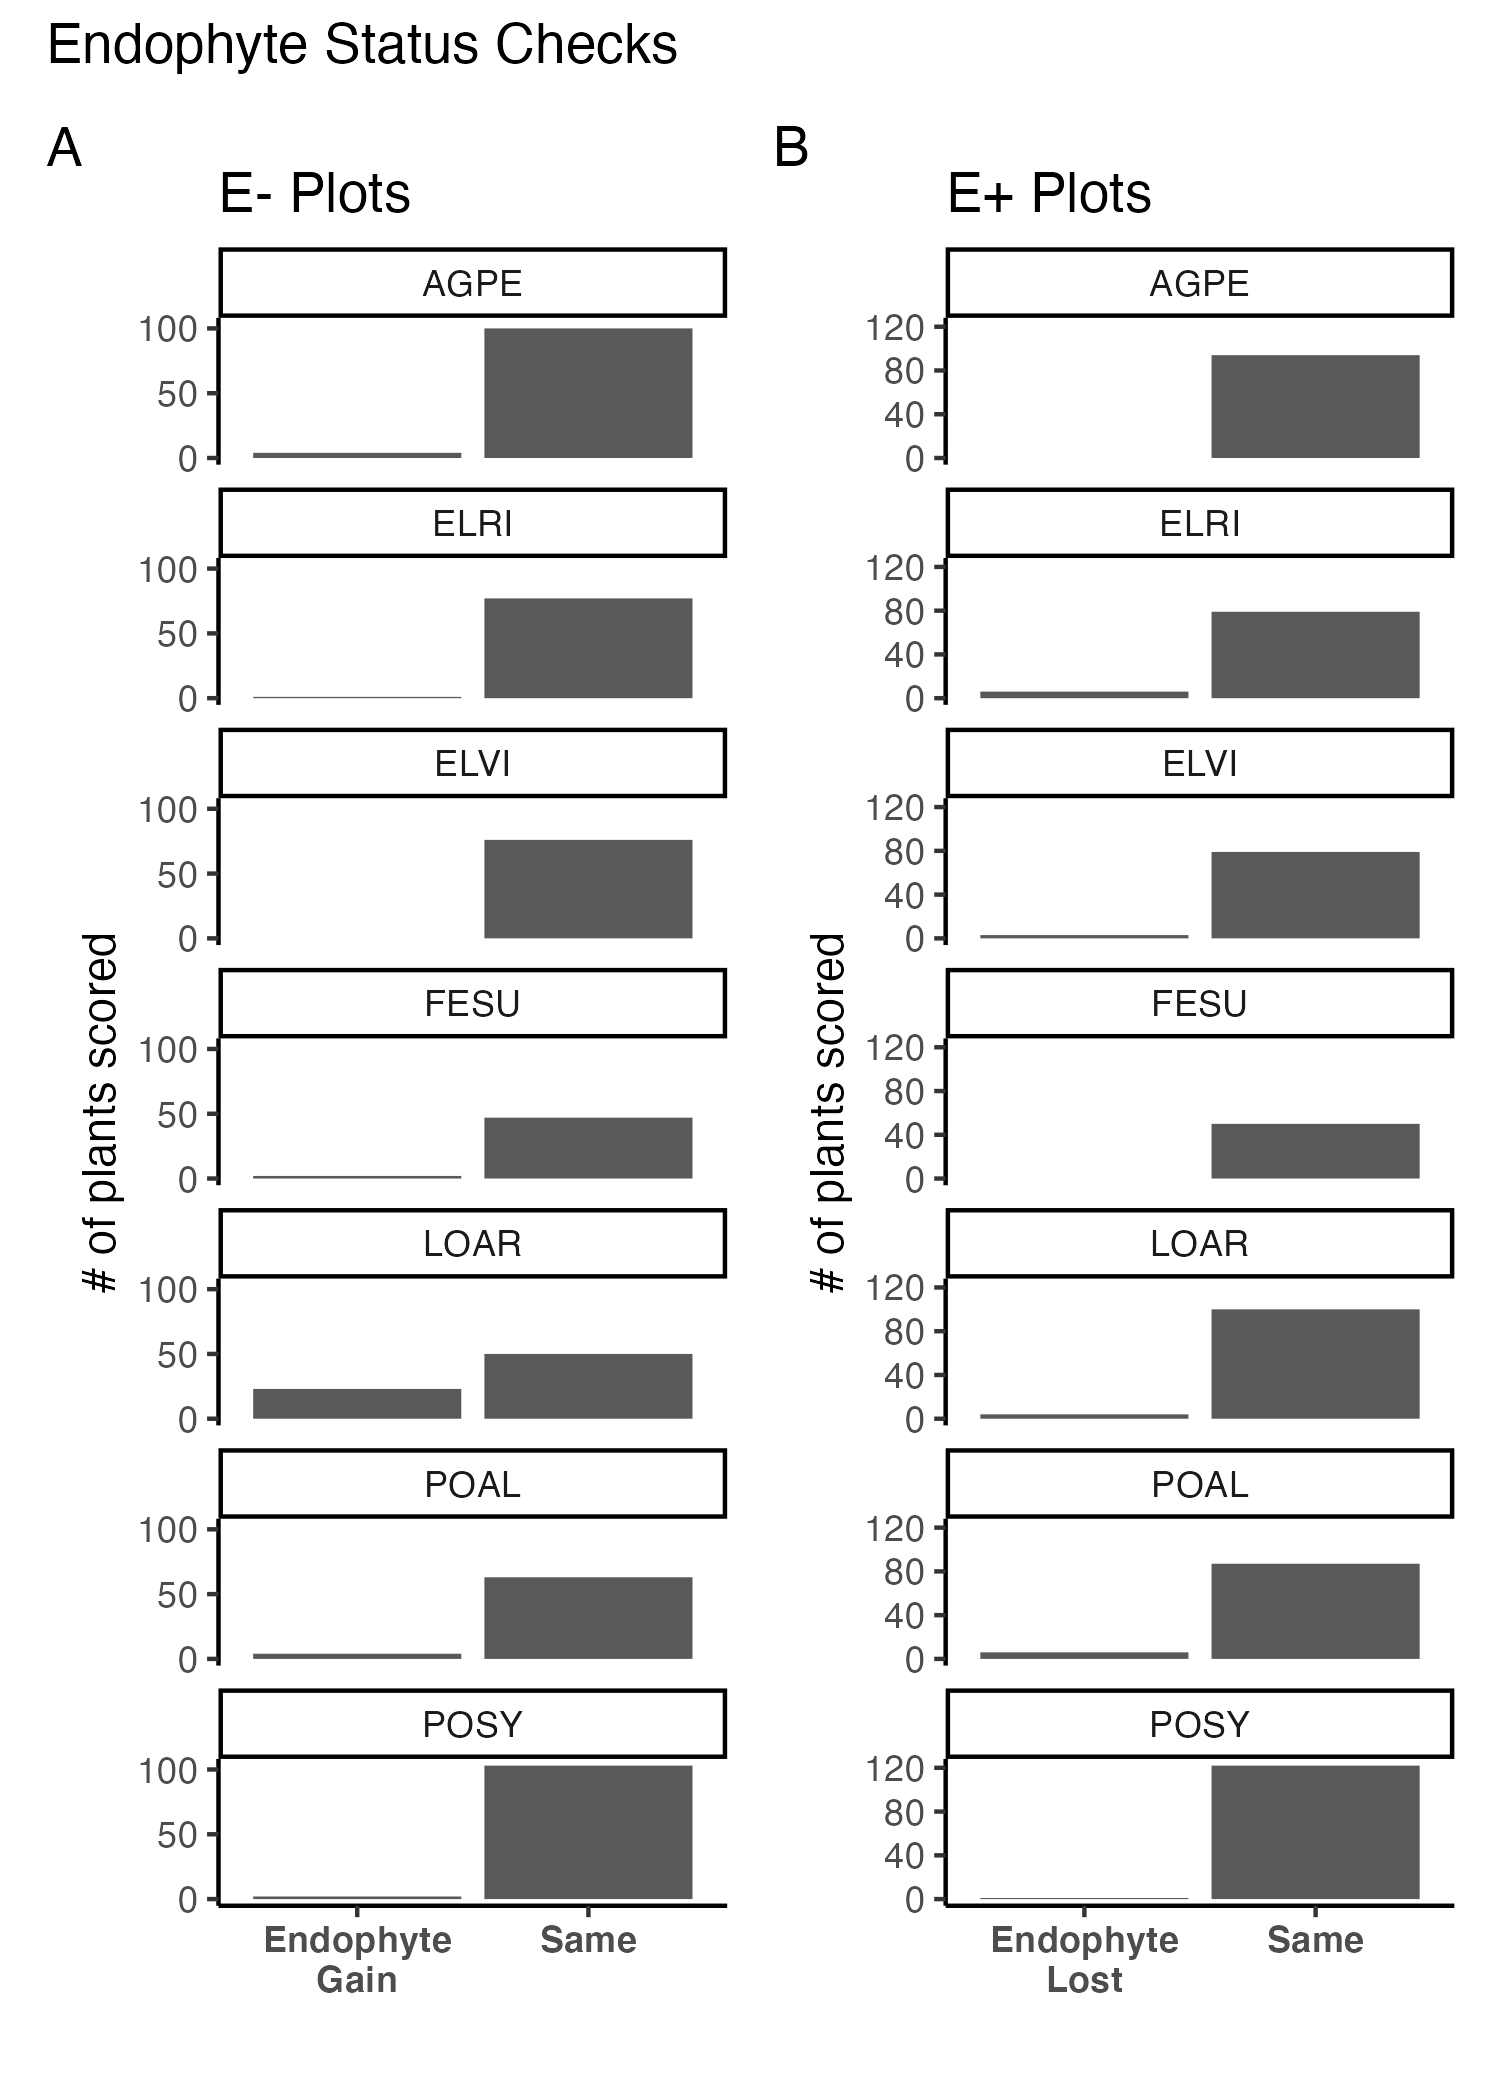
\includegraphics[width=.6\linewidth]{figS8_endo_check_plot.png}
\end{figure}
\noindent {\bf Fig. S8.} \textbf{Faithfulness of experimental plots to assigned endophyte status.} Counts of plants scored with leaf peels or seed squashes to check the faithfulness of recruits to the assigned plot-level endophyte status. (A) Endophytic plants may be gained in initially E- plots, or (B) lost in initially E+ plots.
\newpage

\begin{figure}
	\centering
	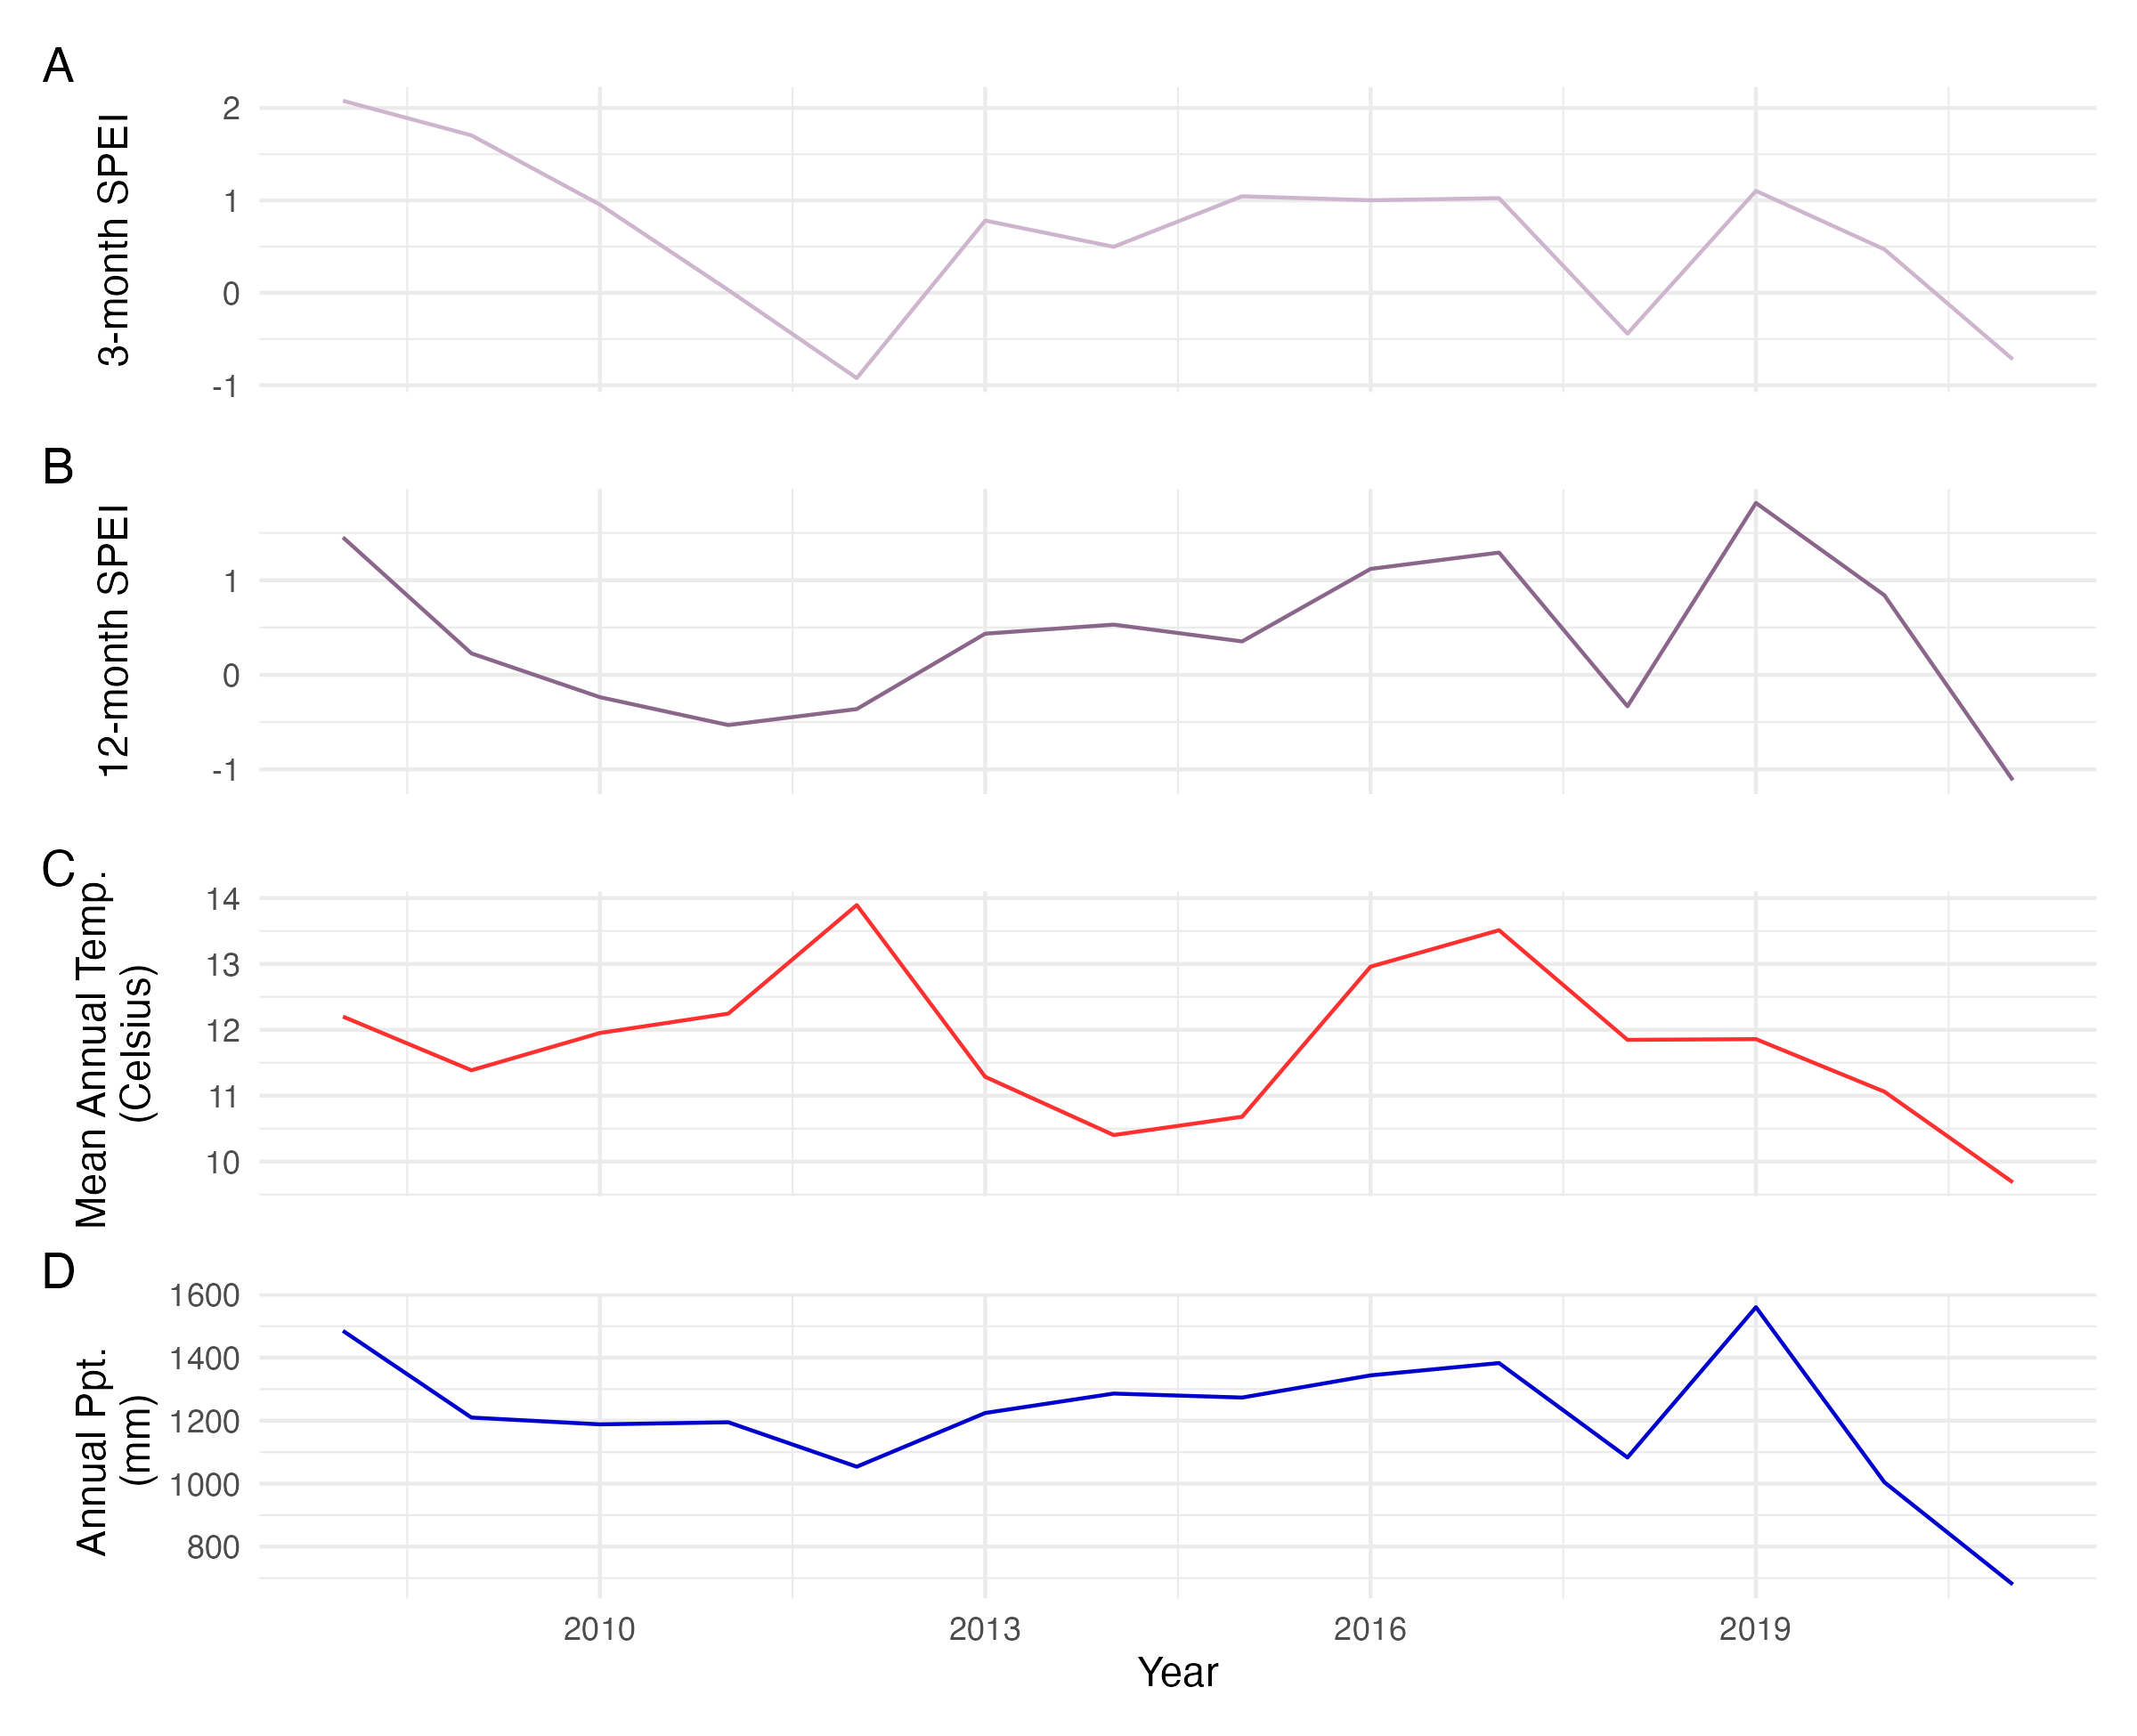
\includegraphics[width=\linewidth]{figS9_climate_plot.png}
\end{figure}
\noindent {\bf Fig. S9.} \textbf{Weather station time-series for Bloomington, IN.} The Seasonal Precipitation-Evapotranspiration Index (SPEI) calculated for the (A) three month growing season and (B) annually from daily weather station observations of (C) average temperatures and (D) cumulative preciptation. Climatic data shown are determined by the census year centered on the month of July. % when \emph{E. villosus} and \emph{E. virginicus}.
\newpage

\begin{figure}
	\centering
	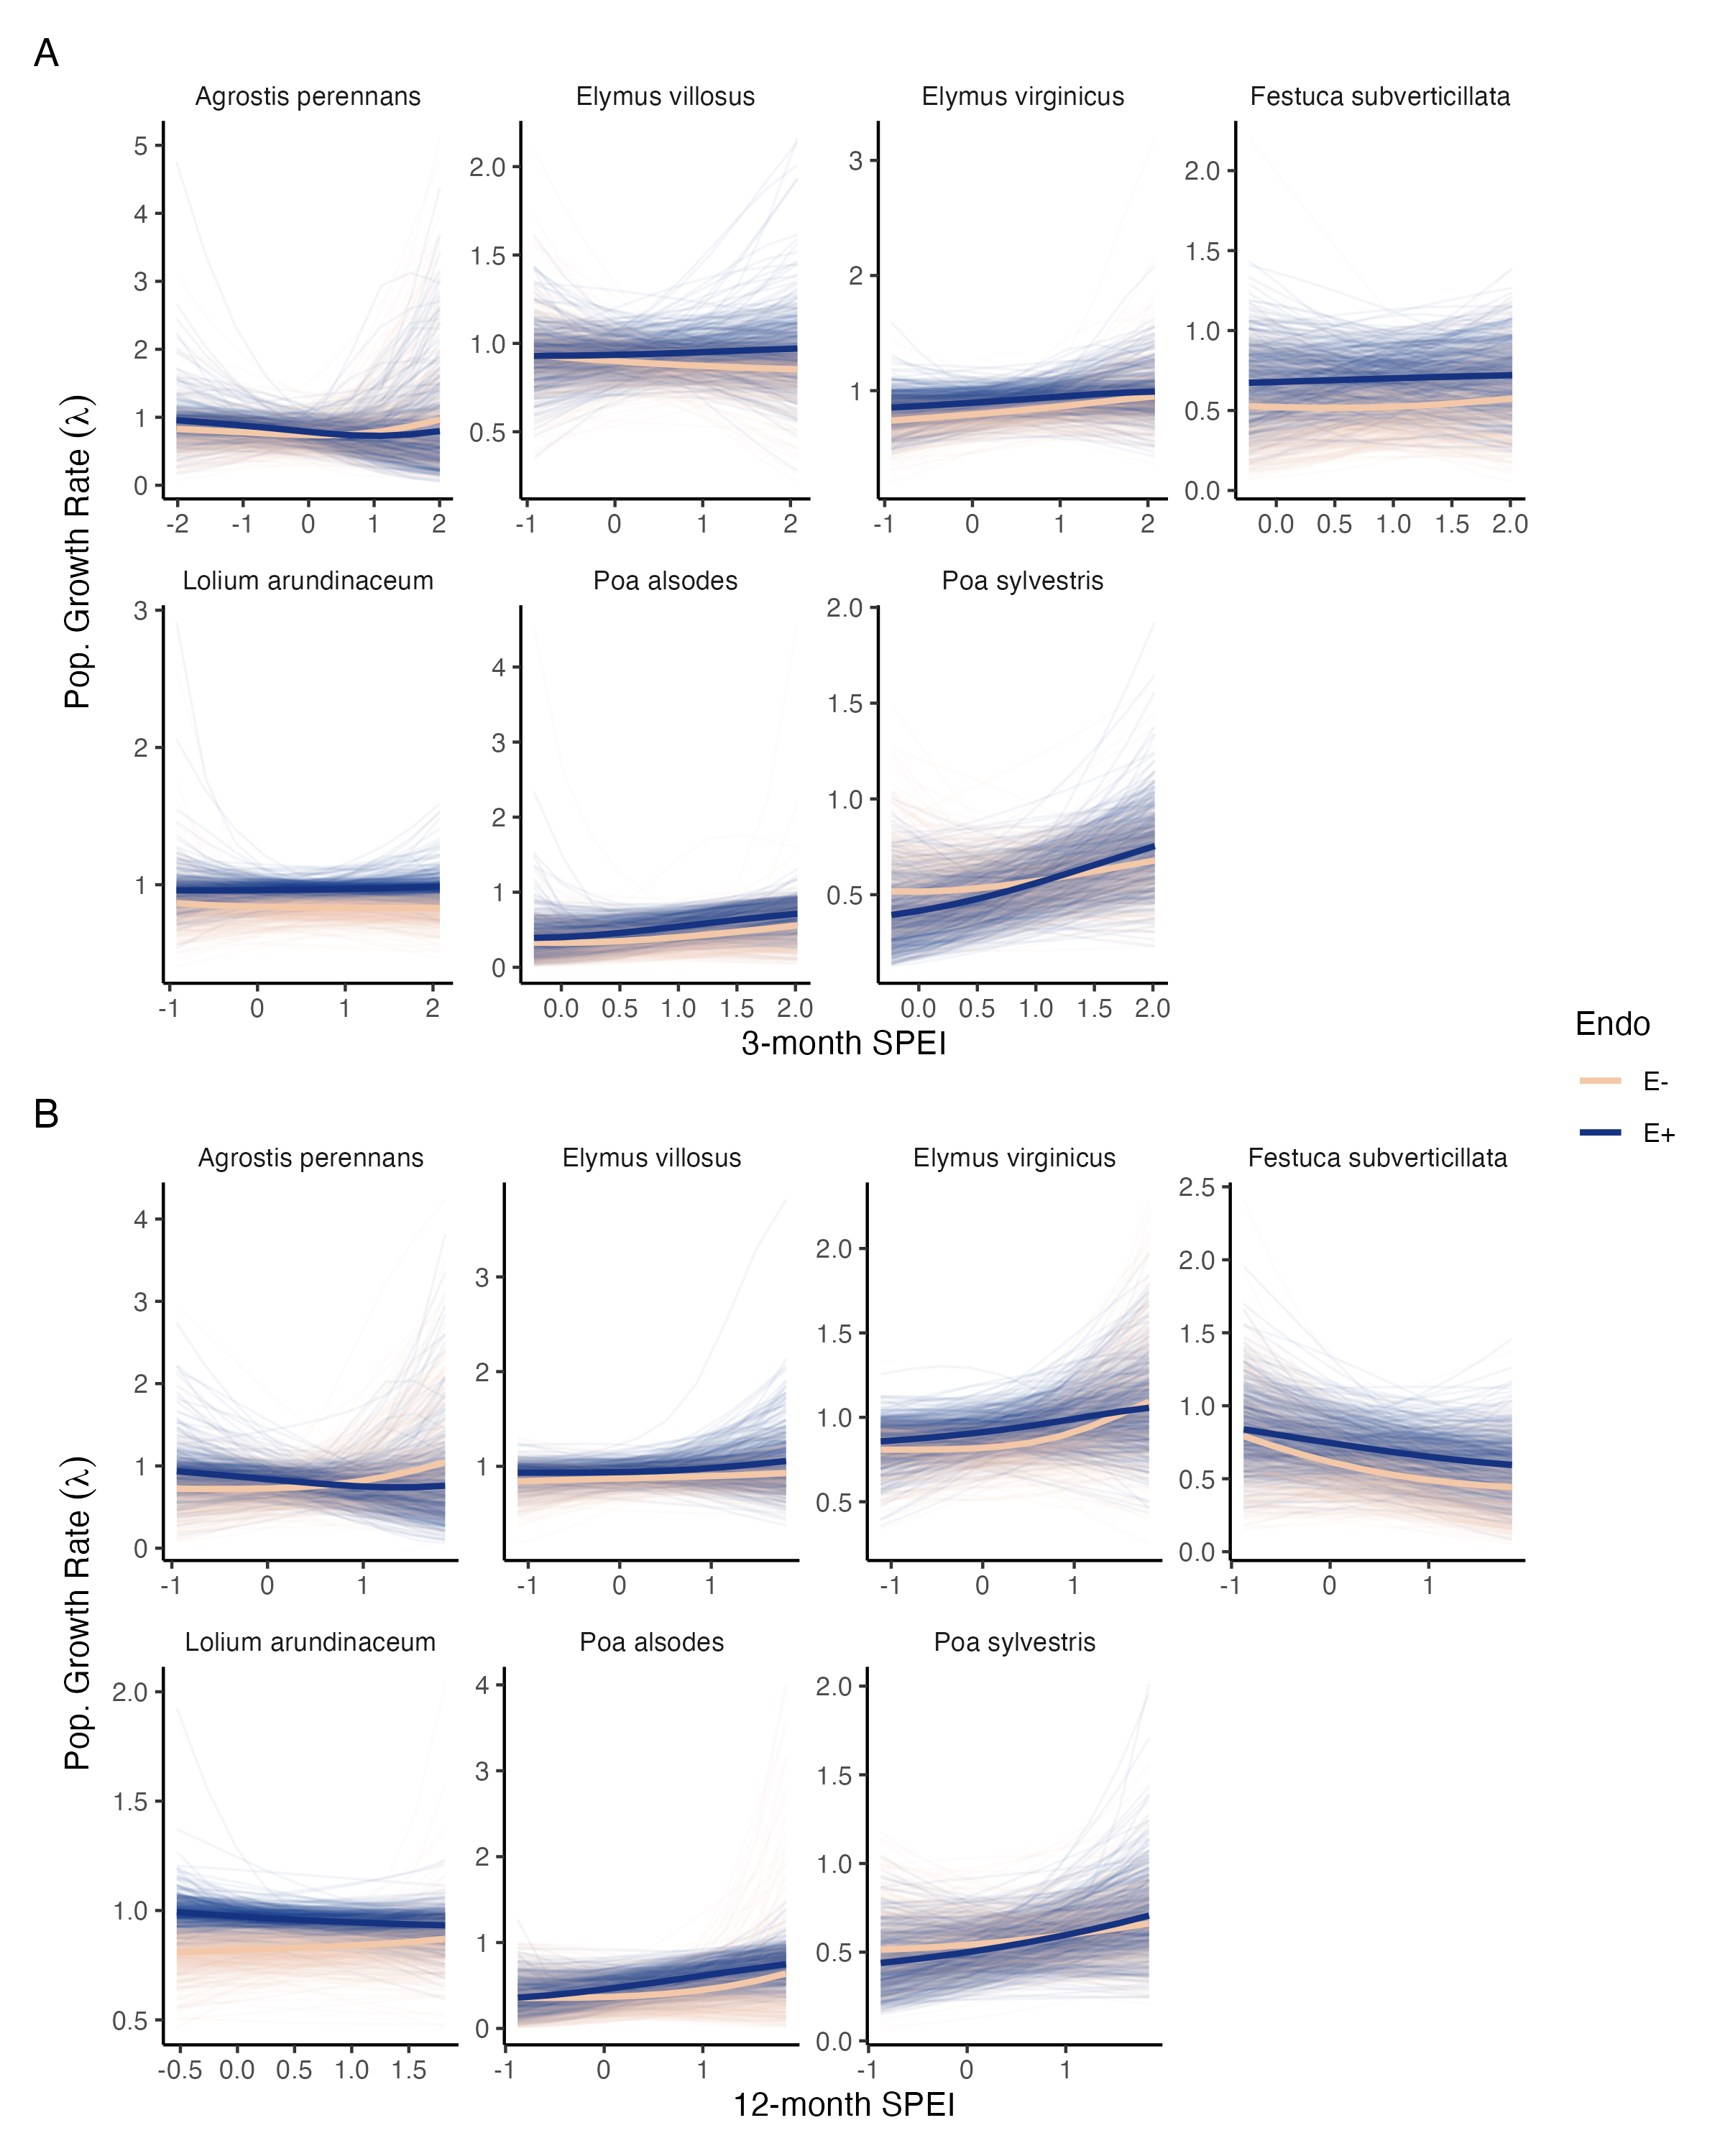
\includegraphics[width=.7\linewidth]{figS10_spei_combo_lambda_plot.png}
\end{figure}
\noindent {\bf Fig. S10.} \textbf{Predicted population growth rates across environmental conditions.} Symbiotic (E+; blue) and symbiont-free (E-; tan) populations respond differently to climate as measured by the (A) 3-month SPEI and (B) 12-month SPEI. Thick lines represent the predicted mean growth rate and thin lines show 500 posterior draws.
\newpage

\noindent {\bf Table S1.} Summary of host-endophyte proprogation and transplant methods\\
\begin{table}[ht]
	\begin{adjustbox}{width=1\textwidth}
\begin{tabular}{llll}

	\bf{Host Species} & \bf{Symbiont Species} & \bf{Heat treatment duration (Temp.)}& \bf{Transplant date }\\
	        \hline
	\emph{Agrostis perennans} & \emph{E. amarillans}&12 min. hot water bath (60 $^{\circ}$C)&\\
	\emph{Elymus villosus}, &\emph{E. elymi}&6 days drying oven (60 $^{\circ}$C)&\\
	\emph{Elymus virginicus} &\emph{E. elymi or EviTG-1}&6 days drying oven (60 $^{\circ}$C)&\\
	 \emph{Festuca subverticillata} &\emph{E. starrii}&6 days drying oven (60 $^{\circ}$C)&\\
	 \emph{Lolium arundinaceum}, &\emph{E. coenophiala}&6 days drying oven (60 $^{\circ}$C)& \\
	 \emph{Poa alsodes} &\emph{E. alsodes}& 7 days drying oven (60 $^{\circ}$C)&\\
	 \emph{Poa sylvestris}&\emph{E. PsyTG-1}&7 days drying oven (60 $^{\circ}$C)& \\
\end{tabular}
\end{adjustbox}
\end{table}


%\tom{(6d in a drying oven at 60$^{\circ}$ C for \emph{E. villosus}, \emph{E. virginicus}, \emph{F. subverticillata},  and \emph{L. arundinaceum}; 7d in a drying oven at 60$^{\circ}$ C for \emph{P. alsodes}, and \emph{P. sylvestris}; and 12 min. in a hot water bath at 60$^{\circ}$ C for \emph{A. perennans})}{need to double check methods for temp, duration, etc.}

\newpage


\noindent {\bf Table S2.} Summary of host-endophyte life history and transmission traits\\
\begin{table}[ht]
\begin{adjustbox}{width=1\textwidth}{
\begin{tabular}{|p{4cm}| p{2cm} |p{2cm}|p{2cm}| p{1cm}|p{2cm}|p{2cm}|p{2cm}|p{2.5cm}| p{2cm}|}
	\hline
	\bf{Host Species} & \bf{Observed max age}& \bf{99th perc. max age}&\bf{Generation time} & $\textbf {R}_0$ &\bf{Longevity}&\bf{Mean life expect.}&\bf{Seed Length (mm.)}&\bf{Imperfect transmission rate} & \bf{Stromata Observed}\\
	\hline
	\emph{Agrostis perennans} &12&7&8.9&0.58&8.5&2.4&1.75&69.8&No\\
	\emph{Elymus villosus}, &14&14&19.5&0.61&14.5&3.4&7.25&100&Yes\\
	\emph{Elymus virginicus} &14&13.6&13.0&0.44&13.5&3.6&8&100&Yes\\
	\emph{Festuca subverticillata} &11&6&7.1&0.47&5.5&1.8&3.75&42.7&No\\
	\emph{Lolium arundinaceum} &12*&12*&30.4&0.57&43.3&12.1&7&100&No\\
	\emph{Poa alsodes} &11&6&10.1&0.004&2.7&1.3&3.45&99.9&No\\
	\emph{Poa sylvestris}&13&6&7.9&0.13&3.2&1.3&2.6&16.6&Yes\\
	 \hline
\end{tabular}}
\end{adjustbox}
\end{table}

* Censuses for \emph{L. arundinaceum} plots stopped after year 12 of the experiment.

\newpage
\noindent {\bf Table S3.} Summary of host-endophyte climate relationships\\
\begin{table}[ht]
	\begin{adjustbox}{width=1\textwidth}{
			\begin{tabular}{|p{4cm}| p{2cm} |p{2cm}|p{2cm}|p{2cm}| p{2cm}|p{2cm}|p{2cm}|p{2cm}|}
				\hline
				\bf{Host Species} & \bf{Effect on CV($\lambda$)}& \bf{Effect on Mean($\lambda$)}&$\frac{\Delta\lambda_{E-}}{\Delta SPEI_{3}}$ & $\frac{\Delta\lambda_{E+}}{\Delta SPEI_{3}}$ &\bf{3 month E- to E+ ratio}&$\frac{\Delta\lambda_{E-}}{\Delta SPEI_{12}}$ &$\frac{\Delta\lambda_{E+}}{\Delta SPEI_{12}}$ &\bf{12 month E- to E+ ratio}\\
				\hline
				\emph{Agrostis perennans} &-0.02641&0.04412&0.0341&-0.0400&0.85&0.11410&-0.06255&1.82\\
				\emph{Elymus villosus}, &0.00033&0.05089&-0.0267&0.0137&1.95&0.02968&0.04216&0.70\\
				\emph{Elymus virginicus} &0.01201&0.05775&0.0697&0.0465&1.50&0.09677&0.06803&1.42\\
				\emph{Festuca subverticillata} &-0.06225&0.16393&0.0213&0.0212&1.01&-0.12873&-0.09010&1.43\\
				\emph{Lolium arundinaceum} &-0.01188&0.10215&-0.0119&0.0090&1.32&0.02644&-0.02596&1.02\\
				\emph{Poa alsodes} &-0.11798&0.12816&0.1017&0.1429&0.712&0.10457&0.14328&0.73\\
				\emph{Poa sylvestris}&-0.02981&-0.00852&0.0717&0.1600&0.44&0.05445&0.09820&0.55\\
				\hline
		\end{tabular}}
	\end{adjustbox}
\end{table}



\end{document}





















